\documentclass[twocolumn, 11pt, draft]{article}
\usepackage{amsmath,amssymb}
\usepackage[format=hang,labelfont=bf,textfont=small,singlelinecheck=false,justification=raggedright,margin={20pt,20pt},figurename=Fig.]{caption}
\usepackage[utf8]{inputenc}
\usepackage[T1]{fontenc}
\usepackage{graphicx}
\usepackage{grffile}
\usepackage{longtable}
\usepackage{wrapfig}
\usepackage{rotating}
\usepackage[normalem]{ulem}
\usepackage{amsmath}
\usepackage{textcomp}
\usepackage{amssymb}
\usepackage{capt-of}
\usepackage{hyperref}
\usepackage{threeparttable}
\usepackage[numbers]{natbib}
\newcommand{\mean}[1]{$\overline{\mbox{#1}}$}
\newcommand{\median}[1]{$\hat{\mbox{#1}}$}

\title{Combining network-guided GWAS to discover susceptibility mechanisms for breast cancer}
\author{Héctor Climente-González$^{1,2,3}$, Christine Lonjou$^{1,2,3}$, Fabienne Lesueur$^{1,2,3}$, \\
GENESIS Study collaborators, Dominique Stoppa-Lyonnet$^{4,5,6}$, \\
Nadine Andrieu$^{1,2,3}$, Chloé-Agathe Azencott$^{3,1,2}$}
\date{$^{1}$Institut Curie, PSL Research University, F-75005 Paris, France;\\
  $^{2}$INSERM, U900, F-75005 Paris, France;\\
  $^{3}$MINES ParisTech, PSL Research University, CBIO-Centre for Computational Biology, F-75006 Paris, France;\\
  $^{4}$Service de Génétique, Institut Curie, F-75005 Paris, France;\\
  $^{5}$INSERM, U830, F-75005 Paris, France;\\
  $^{6}$Université Paris Descartes.\\
}
\hypersetup{
  pdfauthor={Héctor Climente-González, Christine Lonjou, Fabienne Lesueur, GENESIS Study collaborators, Dominique Stoppa-Lyonnet, Nadine Andrieu, Chloé-Agathe Azencott},
  pdftitle={Combining network-guided GWAS to discover susceptibility mechanisms for breast cancer},
  pdfkeywords={},
  pdfsubject={},
  pdflang={English}}
\begin{document}

\onecolumn
\maketitle

\begin{abstract}
Systems biology provides a comprehensive approach to biomarker discovery and biological hypothesis building. It does so by jointly considering the statistical association between gene variation and a phenotype, and the biological context of each gene, represented as a network. In this work, we study the utility of six network methods to discover new biomarkers for breast cancer susceptibility by searching subnetworks with higher association scores to this phenotype. We interrogate a familial breast cancer genome-wide association study focused on \emph{BRCA1/2} negative French women. We perform an in-depth benchmarking of the methods with regards to size of the solution subnetwork, their utility as biomarkers, and the stability and the runtime of the methods. Interestingly, a combination of solution subnetworks provided a concise subnetwork of 93 genes, enriched in known breast cancer susceptibility genes (\emph{BABAM1}, \emph{BLM}, \emph{CASP8}, \emph{FGFR2}, and \emph{TOX3}, Fisher's exact test P-value = $7.8 \times 10^{-5}$ ) and occupy more central positions in the network than average. Additionally, it includes subnetworks of mechanisms related to cancer, like protein folding (\emph{HSPA1A}, \emph{HSPA1B}, and \emph{HSPA1L}) or mitochondrial ribosomes (\emph{MRPS30}, \emph{MRPS31}, \emph{MRPS18B}). We also observed a general dysregulation in the neighborhood of \emph{COPS5}, a gene related to multiple hallmarks of cancer. By trading statistical astringency for biological meaningfulness, most network methods get more compelling results than standard SNP- and gene-level analyses, recovering causal subnetworks tightly related to cancer susceptibility. 
\end{abstract}

\section{Introduction}

In human health, genome-wide association studies (GWAS) aim at quantifying how single-nucleotide polymorphisms (SNPs) predispose to complex diseases, like diabetes or some forms of cancer \cite{bush_chapter_2012}. To that end, in a typical GWAS thousands of unrelated samples are genotyped: the cases, suffering the disease of interest, and the controls from the general population. Then, a per-SNP statistical association test is conducted (e.g. logistic regression). Those SNPs with a P-value lower than a conservative Bonferroni threshold are candidates to further studies in an independent cohort. Once the risk SNPs have been discovered, they can be used for risk assessment, and to deepen our understanding of the disease.

GWAS have successfully identified thousands of variants underlying many common diseases \cite{buniello_nhgri-ebi_2019}. However, the experimental setting also presents intrinsic challenges. Some of them stem from the high-dimensionality of the problem, as every GWAS to date studies more variants than samples are genotyped. This limits the statistical power of the experiment, as only variants with large and moderate effects can be detected. And it is particularly problematic since the prevailing view is that most genetic architectures involve many variants with small effects \cite{visscher_10_2017}. Additionally, to avoid false positives, a conservative multiple test correction is applied, typically Bonferroni. However, Bonferroni is known to be overly conservative when the statistical tests are correlated, as is the case in GWAS \cite{wang_statistical_2018}. Another open issue is the interpretation of the results, as the functional consequences of most common variants are not well understood. On top of that, recent large-sampled studies suggest that most of the genome contributes to a degree to any complex trait, in accordance with the infinitesimal model \cite{barton_infinitesimal_2017}. The recently proposed omnigenic model \cite{boyle_expanded_2017} offers an explanation: genes are very functionally inter-related and influence each other's behavior, which allows alterations in most genes to impact the subset of ``core'' genes directly involved in a disease's mechanism. Hence, a comprehensive statistical framework which includes the structure of biological data might address the aforementioned issues.

In this regard many authors turn to network biology to handle the complex interplay of biomolecules that lead to disease \cite{furlong_human_2013}. As its name suggests, network biology models biology as a network, where the biomolecules under study, often genes, are nodes, and between them are the edges that link them. These functional relationships come from evidence that the genes jointly contribute to a biological function; for instance, their expression is correlated, or their products establish a protein-protein interaction. Under this view, complex diseases are not the consequence of a single altered gene, but of the interaction of multiple interdependent molecules \cite{barabasi_network_2011}. In fact, an examination of biological networks shows that disease genes have differential properties \cite{barabasi_network_2011} \cite{pinero_uncovering_2016}. This is particularly true for cancer driver genes, which tend to be key players in connecting different, densely-connected communities of genes. Additionally, as genes that contribute to a disease tend to participate in similar biological functions, studying the neighborhood of known disease genes is effective at identifying new ones \cite{huang_systematic_2018}. 

Network-based, biomarker discovery methods exploit the aforementioned strategy to identify disease genes on GWAS data \cite{azencott_network-guided_2016}. In essence, each SNP has a score of association with the disease, given by the experiment, and functionally biological relationships, given by a network built on prior knowledge. Then, the problem becomes finding a functionally-related set of highly-scoring genes. Different solutions have been proposed to this problem, often stemming from divergent different mathematical frameworks and considerations of what the optimal solution looks like. Some methods strongly constrain the problem to certain kinds of subnetworks. Such is the extreme case of LEAN \cite{gwinner_network-based_2016}, which focuses on star subnetworks, i.e. instances were both a gene and its direct interactors are associated with the disease. Other algorithms, like dmGWAS \cite{jia_dmgwas:_2011} and heinz \cite{dittrich_identifying_2008}, focus on interconnected genes with high association with the disease. However, they differ in their tolerance to the inclusion of low scoring nodes, and the possible number of disconnected subnetworks in the solution. Lastly, other methods also consider the topology of the network, favoring solutions that are densely interconnected; such is the case of HotNet2 \cite{leiserson_pan-cancer_2015}, SConES \cite{azencott_efficient_2013}, and SigMod \cite{liu_sigmod:_2017}.

In this work, we analyze the effectiveness of these six network methods for biomarker discovery on GWAS data. While all of them capture susceptibility mechanisms resembling that postulated by the omnigenic model, they do so in different ways, and provide a representative view of the field. We focus on the GENESIS dataset \cite{sinilnikova_genesis:_2016}, a study of familial breast cancer conducted in the French population. After a classical GWAS approach, we use these network-based methods to recover additional breast cancer biomarkers. Lastly, we carry out a comparison of the solutions obtained by the different methods, and aggregate them to obtain a consensus network of predisposition to familial breast cancer. 

\section{Methods}
\subsection{GENESIS}

The GENE Sisters (GENESIS) study was designed to investigate risk factors for familial breast cancer in the French population \cite{sinilnikova_genesis:_2016}. Index cases are patients with infiltrating mammary or ductal adenocarcinoma, who had a sister with breast cancer, and who have been tested negative for \emph{BRCA1} and \emph{BRCA2} pathogenic variants. Controls are unaffected colleagues and/or friends of the cases, born around the year of birth of the corresponding case (\textpm{} 3 years). We focused on the 2\,577 samples of European ancestry, of which 1\,279 are controls and 1\,298 are cases. The genotyping was performed using the iCOGS array, a custom Illumina array designed to study genetic susceptibility of hormone-related cancers \cite{sakoda_turning_2013}. It contains 211\,155 SNPs, including SNPs putatively associated with breast, ovarian, and prostate cancers, SNPs associated with survival after diagnosis, and SNPs associated to other cancer-related traits, as well as functional candidate variants in selected genes and pathways.

\subsection{Preprocessing and quality control}

We discarded SNPs with a minor allele frequency lower than 0.1\%, those not in Hardy - Weinberg equilibrium in controls (P-value \textless 0.001), and those missing on more than 10\% of the samples. A subset of 20 duplicated SNPs in \emph{FGFR2} were also removed. In addition, we removed the samples with more than 10\% missing genotypes. After control for relatedness, 17 additional samples were removed (6 for sample identity error, 6 false ``friend/control'' having family link with other samples, 3 ``friend/control'' having a high relatedness score). Lastly, based on study selection criteria, 11 other samples were removed (1 control having cancer, 4 index cases with no affected sister, 3 half-sisters, 1 sister with CLIS, 1 with \emph{BRCA1/2} mutation detected in the family, 1 with molecular diagnosis not received). The final dataset included 1\,271 controls and 1\,280 cases, genotyped over 197\,083 SNPs. 

We looked for population structure that could create confounding associations. A PCA revealed no visual differential population structure between cases and controls (Supplementary Figure \ref{sfig:pcs}). Independently, we did not find evidence of genomic inflation (\(\lambda\) = 1.05) either, further confirming the absence of confounding population structure.

\subsection{High-score subnetwork search algorithms}
\subsubsection{SNP and gene association}
\label{methods:node_score}
To measure association between a genotype and the phenotype, we performed a per-SNP 1~d.f.~\(\chi\)\textsuperscript{2} allelic test using PLINK v1.90 \cite{chang_second-generation_2015}. Then, we used VEGAS2v2 to compute the gene-level association score \cite{mishra_vegas2:_2015} from the SNP P-values. In order to map SNPs to genes we used their overlap on the genome: all SNPs located within the boundaries of a gene, \textpm 50 kb, were mapped to that gene. To compute the gene association score we used the 10\% of SNPs linked to the gene with lowest P-values. We used the 62\,193 genes described in GENCODE 31 \cite{frankish_gencode_2019}, although only 54\,612 could be mapped to at least one SNP. Out of those, we focused exclusively on the 32\,767 that had a gene symbol. Out of the SNPs 197\,083 remaining after quality control, 164\,037 were mapped to at least one of these genes. 

We use such mapping to compare the outputs of methods that produce SNP- to those that produce gene-lists, and vice versa. In the former case, we consider any gene that can be mapped to any of the selected SNPs as selected as well. In the latter, we consider all the SNPs that can be mapped to that gene as selected by the method.

\subsubsection{Mathematical notation}
\label{methods:notation}
In this article, we use undirected, vertex-weighted networks, or graphs, $G = (V,E,w)$. $V = \{v_{1}, \dots{}, v_{n}\}$ refers to the vertices, with weights $w: V \rightarrow \mathbb{R}$. Equivalently, $E \subseteq \{\{x,y\} | x,y \in V \wedge x \neq y\}$ refers to the edges. When referring to a subnetwork S, $V_{S}$ is the set of nodes in S and $E_{S}$ is the set of edges in S. A special case of subgraphs are \emph{connected} subgraphs, which occur when every node in the subgraph can be reached from any other node.

On top of a weight, nodes have other properties provided by the topology of the graph. In this article we focus on two: degree centrality, and betweenness centrality. The degree centrality, or degree, is the number of edges that a node has. The betweenness centrality, or betweenness, is the number of times a node participates in the shortest paths between two other nodes.

In addition, we use several matrices that describe different properties of a graph. The described matrices are square, and have as many rows and columns as nodes are in the network. The element $(i,j)$ represents a  selected relationship between $v_i$ and $v_j$. The \emph{adjacency matrix} $W_G$ contains a 1 when the corresponding nodes are connected, and 0 otherwise; the diagonal is zero. The \emph{degree matrix} $D_G$ is a diagonal matrix which contains the degree of the different nodes. Lastly, the \emph{Laplacian matrix} $L_G$ is defined as $L_G = D_G - W_G$.

\subsubsection{Methods used}
\label{methods:methods}

\begin{table}[htbp]
  \caption{\label{tab:method_comparison} Summary of the differences between the studied algorithms.}
  \centering
  \begin{threeparttable}
    \begin{tabular}{l|llllllll}
      Method & Field & Nodes & Exhaustive & Solution & Components & Input & Scoring & Reference\\
      \hline
      dmGWAS & GWAS & Genes & No & - & 1 & Summary & -log\textsubscript{10}(P) & \cite{jia_dmgwas:_2011}\\
      heinz & Omics & Genes & Yes & - & 1 & Summary & BUM & \cite{dittrich_identifying_2008}\\
      HotNet2 & Omics & Genes & Yes & Module & \(\ge\) 1 & Summary & Local FDR & \cite{leiserson_pan-cancer_2015}\\
      LEAN & Omics & Genes & Yes & Star & \(\ge\) 1 & Summary & -log\textsubscript{10}(P) & \cite{gwinner_network-based_2016}\\
      SConES & GWAS & SNPs & Yes & Module & \(\ge\) 1 & Genotypes & \(\chi\)\textsuperscript{2} & \cite{azencott_efficient_2013}\\
      SigMod & GWAS & Genes & Yes & Module & 1 & Summary & -log\textsubscript{10}(P) & \cite{liu_sigmod:_2017}\\
    \end{tabular}
    \begin{tablenotes}
      \item \textbf{\emph{Field}}: field in which the algorithm was developed.\\
      \item \textbf{\emph{Nodes}}: the type of network, either gene (protein-protein interaction network usually) or a SNP network.\\
      \item \textbf{\emph{Exhaustive}}: whether all the possible solutions given the selected hyperparameters are explored.\\
      \item \textbf{\emph{Solution}}: additional properties are enforced on the solution subnetwork, other than being dense in high scores and connected.\\
      \item \textbf{\emph{Components}}: number of connected subnetworks in the solution.\\
      \item \textbf{\emph{Input}}: genotype data or GWAS summary statistics.\\
      \item \textbf{\emph{Scoring}}: how SNP/gene P-values are transformed into node scores.\\
      \item \textbf{\emph{Reference}}: original publication featuring the algorithm.
    \end{tablenotes}
  \end{threeparttable}
\end{table}

Beyond the assumption that genes that contribute to the same function will be nearby in the protein-protein interaction network (PPIN), they might be topologically related to each other in diverse ways (densely interconnected modules, nodes around a hub, a path, etc.). That is not the only choice to make: how to score the nodes, whether the affected mechanisms form a single connected component or several, how to frame the problem in a computationally efficient fashion, what is the best network to use, etc. In consequence, multiple solutions have been proposed. In this article, we examine six of them: five that explore the PPIN, and one which explores SNP networks. We selected methods that were open source, had an implementation available, and an accessible documentation. Their main differences are summarized in Table \ref{tab:method_comparison}.

\begin{description}
\item[{dmGWAS}] dmGWAS searches the subgraph with the highest local density in low P-values \cite{jia_dmgwas:_2011}. To that end it searches candidate subnetwork solutions using a greedy, ``seed and extend'', heuristic:

\begin{enumerate}
\item Select a seed node.
\item Compute Stouffer's Z-score Z\textsubscript{m} for the current subgraph $S$ as

\begin{equation*} 
Z_m = \frac{\sum_{i \in S} z_i}{\sqrt{k}}
\end{equation*}

where \emph{k} is the number of genes in the subgraph; z\textsubscript{i} is the score of gene $i$, computed as \(\phi\)\textsuperscript{-1}(1 - P-value\textsubscript{i}); and \(\phi\)\textsuperscript{-1} is the inverse normal distribution function.
\item Identify neighboring nodes i.e. nodes at distance \(\le\) \emph{d}. We set d = 2.
\item Add the neighboring nodes whose inclusion increases the Z\textsubscript{m+1} more than Z\textsubscript{m} \texttimes{} (1 + r). In our experiments, we set r = 0.1.
\item Repeat 2-4 until no increment Z\textsubscript{m} \texttimes{} (1 + r) is possible.
\end{enumerate}

Lastly, the module's Z-score is normalized as

\begin{equation*}
Z_{N}=\frac{Z_{m}-\operatorname{mean}\left(Z_{m}(\pi)\right)}{\operatorname{SD}\left(Z_{m}(\pi)\right)}
\end{equation*} 

where Z\textsubscript{m}(\(\pi\)) represent a vector containing 100\,000 random subsets of the same number of genes.

We used the implementation of dmGWAS in the dmGWAS 3.0 R package \cite{dmgwas}. We used the function \emph{simpleChoose} to select the solution subnetwork, which aggregates the top 1\% modules into the solution subnetwork.
\end{description}

\begin{description}
\item[{heinz}] The goal of heinz is to identify the highest-scored connected subgraph on the network \cite{dittrich_identifying_2008}. The authors propose a transformation of the genes' P-value into a score that is negative under no association with the phenotype, and positive value when there is. This transformation is achieved by modelling the distribution of P-values by a beta-uniform model (BUM) parameterized by the desired FDR. Thus formulated, the problem is NP-complete, and hence solving it would require a prohibitely long computational time. To solve it efficiently it is re-casted as the Prize-Collecting Steiner Tree Problem (PCST), which seeks to select the connected subnetwork S that maximizes the \emph{profit} p(S):

\begin{equation*}
p(S) = \sum_{v \in V_S} p(v) - \sum_{e \in E_S} c(e). 
\end{equation*}

were p(v) = w(v) - w' is the \emph{profit} of adding a node, c(e) = w' is the \emph{cost} of adding an edge, and $w' = min_{v \in V_{G}} w(v)$. All three are positive quantities. heinz implements the algorithm from \citet{ljubic_algorithmic_2006}, which in practice is often fast and optimal, neither is guaranteed. We used BioNet's implementation of heinz, available on Bioconductor \cite{beisser_bionet:_2010,heinz}.

\item[{HotNet2}] HotNet2 was developed to find connected subgraphs of genes frequently mutated in cancer \cite{leiserson_pan-cancer_2015}. To that end, it considers both the local topology of the network and the scores of the nodes. The former is captured by an insulated heat diffusion process: at the beginning, the score of the node determines its initial heat; iteratively each node yields heat to its ``colder'' neighbors, and receives heat from its ``hotter'' neighbors, while retaining part of its own (hence, \emph{insulated}). This process continues until equilibrium is reached, and results in a similarity matrix F. F is used to compute the similarity matrix E that accounts also for similarities in node scores as 

\begin{equation*} 
E = F \operatorname{diag}(w(V)), 
\end{equation*}

where $\operatorname{diag}(w(V))$ is a diagonal matrix with the node scores in its diagonal. We scored the nodes as in \citet{nakka_gene_2016}, assigning a score of 0 for the genes with low probability of being associated to the disease, and -log\textsubscript{10}(P-value) to those likely to be. In this dataset, the threshold separating both was a P-value of 0.125, which was obtained using a local FDR approach \cite{scheid_twilight;_2005}. To obtain densely connected subnetworks, HotNet2 prunes E, only preserving edges such that w(E) \textgreater{} \(\delta\). Lastly, HotNet2 evaluates the statistical significance of the subnetworks by comparing their size to the size of networks obtained by permuting the node scores. HotNet2 has two parameters: the restart probability \(\beta\), and the threshold heat \(\delta\). Both parameters are set automatically by the algorithm, and are robust \cite{leiserson_pan-cancer_2015}. HotNet2 is implemented in Python \cite{hotnet2}.

\item[{LEAN}] LEAN searches disregulated ``star'' gene subnetworks, that is, subnetworks composed by one central node and all its interactors \cite{gwinner_network-based_2016}. By imposing this restriction, LEAN is able to exhaustively test all such subnetworks (one per node). For a particular subnetwork of size \emph{m}, the P-values corresponding to the involved nodes are ranked as p\textsubscript{1} \(\le\) \dots{} \(\le\) p\textsubscript{m}. Then, \emph{k} binomial tests are conducted, to compute the probability of having \emph{k} out of \emph{m} P-values lower or equal to p\textsubscript{k} under the null hypothesis. The minimum of these \emph{k} P-values is the score of the subnetwork. This score is transformed into a P-value through an empirical distribution obtained via a subsampling scheme, where sets of \emph{m} genes are selected randomly, and their score computed. Lastly, P-values are corrected for multiple testing through a Benjamini-Hochberg correction. We used the implementation of LEAN from the LEANR R package \cite{leanr}.
\item[{SConES}] SConES searches the minimal, modular, and maximally associated subnetwork in a SNP graph \cite{azencott_efficient_2013}. Specifically, it solves the problem

\begin{equation}
\label{eq:scones}
\underset{S \subseteq G}{\arg \max } \underbrace{\sum_{v \in V_S} w(v)}_{\text { association }} + \underbrace{\lambda \sum_{v \in V_S} \sum_{u \not\in V_S} L_{vu} }_{\text { connectivity }}-\underbrace{\eta \lvert V_S \rvert }_{\text { sparsity }}
\end{equation}

where \(\lambda\) and \(\eta\) are hyperparameters that control the sparsity and the connectivity of the model. Given two hyperparameters, the aforementioned problem has a unique solution, that SConES finds using a graph min-cut procedure. We used the version on SConES implemented in the R package martini \cite{martini}. As in \citet{azencott_efficient_2013}, we selected \(\lambda\) and \(\eta\) by cross-validation, choosing the values that produce the most stable solution across folds. Note that the solution to the above problem can consist of several connected subnetworks which are disconnected from each other. In this case, the selected hyperparameters were \(\eta\) = 3.51, \(\lambda\) = 210.29 for SConES GS; \(\eta\) = 3.51, \(\lambda\) = 97.61 for SConES GM; and \(\eta\) = 3.51, \(\lambda\) = 45.31 for SConES GI.
\end{description}

\begin{description}
\item[{SigMod}] SigMod aims at identifying the highest-scoring, most densely connected gene subnetwork \cite{liu_sigmod:_2017}. It addresses an optimization problem similar to that of SConES (Equation \ref{eq:scones}), but using the adjacency matrix rather than the Laplacian matrix (Section \ref{methods:notation}), to quantify solutions containing many edges.  

\begin{equation*}
\underset{S \in G}{\arg \max } \underbrace{\sum_{v \in V_S} w(v)}_{\text { association }} + \underbrace{\lambda \sum_{v \in V_S} \sum_{u \in V_S} W_{vu} }_{\text { connectivity }} -\underbrace{\eta \lvert V_S \rvert }_{\text { sparsity }}.
\end{equation*}

As SConES, this optimization problem can also be solved by a graph min-cut approach. 

SigMod presents three important differences with SConES. First it is designed for gene-gene networks. Second, by replacing the adjacency by the Laplacian matrix, it favors subnetworks containing many edges. SConES, instead, penalizes connections between the selected and unselected nodes. Third, it returns a single connected subnetwork, which it achieves by exploring a grid of hyperparameters and processing their respective solutions. Specifically, for the range of \(\lambda\) = \(\lambda\)\textsubscript{min}, \dots{}, \(\lambda\)\textsubscript{max} for the same \(\eta\), it prioritizes the solution with the largest change in size from \(\lambda\)\textsubscript{n} to \(\lambda\)\textsubscript{n+1}. Such a large change implies that the network is densely interconnected. This results in one candidate solution for each \(\eta\), which are processed by removing any node not connected to any other. A score is assigned to each candidate solution by summing their node scores and normalizing by size. The candidate solution with the highest standardized score is the chosen solution. SigMod is implemented in an R package \cite{sigmod}.
\end{description}

\begin{description}
\item[{Consensus}] In addition, we built a consensus network by retaining the nodes that were selected by at least two of the six methods (using SConES GI for SConES).
\end{description}

\subsubsection{Gene-gene network}
\label{methods:gene_network}
Out of the six methods tested, five use a gene-gene interaction network (Section \ref{methods:methods}). Although their respective statistical frameworks are compatible with any type of network (protein interactions, gene coexpression, regulatory, etc.), for practical reasons we focused on a PPIN, as they are interpretable, well characterized, and most of the methods were designed to scale appropriately to it. We built our PPIN from both binary and co-complex interactions stored in the HINT database (release April 2019) \cite{das_hint:_2012}. Unless specified otherwise, we used only interactions coming from high-throughput experiments to avoid biasing the topology of the network by well-studied genes with more known interactions on average. Out of the 146\,722 interactions from high-throughput experiments that HINT stores, we were able to map 142\,541 to a pair of gene symbols. The scoring function for the nodes changed from method to method (Section \ref{methods:methods}).

Additionally, we compared the results of the aforementioned PPIN with those obtained on another PPIN built using interactions coming from both high-throughput and targeted studies. In that case, out of the 179\,332 interactions in HINT, we mapped 173\,797 to a pair of gene symbols. 

\subsubsection{SNP networks}
\label{methods:snp_network}
SConES \cite{azencott_efficient_2013} is the only of the studied methods designed to handle SNP networks. As in gene networks, two SNPs are linked in a SNP network when there is evidence of shared functionality between two SNPs. The authors suggested three ways of building these networks: connecting the SNPs consecutive in the genomic sequence (``GS network''); interconnecting all the SNPs mapped to the same gene, on top of GS (``GM network''); and interconnecting all SNPs mapped to two genes for which a protein-protein interaction exists (``GI network''). We focused on the GI network, as it is the network that fits better the scope of this article. However, at different stages of this work we also used GS and GM for comparison. For the GM network, we used the mapping described in Section \ref{methods:node_score}. For the GI network, we used the PPI as described in Section \ref{methods:gene_network}. For all three networks the node score used is an association score of the individual SNPs with the phenotype (1~d.f.~\(\chi\)\textsuperscript{2}).

\subsection{Evaluation of methods}

We evaluated multiple properties of the different method through a 5-fold subsampling setting. We applied each method to 5 random subsets of the original dataset containing 80\% of the samples (\emph{train set}). When pertinent, we evaluated the solution on the remaining 20\% (\emph{test set}). We used the 5 repetitions to estimate the average and the deviation of the different measures.

\subsubsection{Properties ot the solution}
\label{methods:comparison}

We compared the runtime, the number of selected genes/SNPs, and the stability (sensitivity of the result to small changes in the input) of the different network methods. The stability was measured using the Pearson's correlation between different runs as suggested \citet{nogueira_measuring_2016}.

\subsubsection{Classification accuracy of selected biomarkers}
\label{methods:classifier}

A desirable solution offers good predictive power on unseen \emph{test} samples. We evaluated the predicting power of the SNPs selected by the different methods through the performance of an L1-penalized logistic regression classifier trained exclusively on those SNPs to predict the outcome (case/control). The L1 penalty helps to account for LD by reducing the number of SNPs included in the model (size of the active set), while improving the generalization of the classifier. This penalty was set by cross-validation. We applied each network method to each \emph{train} set, and trained the classifier on the \emph{train} set as well using only on the selected SNPs. When the method retrieved a list of genes (all of them except SConES), we considered as selected all the SNPs mapped to any of those genes. Then we evaluated the sensitivity and the specificity on the \emph{test set}. To obtain a baseline, we also trained the classifier on all the SNPs. We also evaluated the size of the active set, an estimate of a plausible, more sparse solution with a comparable predictive power to the original solution.

\subsubsection{Comparison to state-of-the-art}
\label{methods:bcac}
An alternative way to evaluate the results is comparing our results to an external dataset. For that purpose, we recovered a list of 153 genes associated to familial breast cancer from DisGeNET \cite{pinero_disgenet:_2017}. Across this article we refer to these genes as \emph{breast cancer susceptibility genes}.

Additionally, we used the summary statistics from the Breast Cancer Association Consortium (BCAC), a meta-analysis of case-control studies conducted in multiple countries which included 228\,951 women of European ancestry from the general population \cite{Michailidou2017}. Hence, a high proportion of breast cancer cases investigated in BCAC are sporadic, while GENESIS is a homogeneous dataset focusing on the French high-risk population attending the family cancer clinics. Despite these differences, there should be shared genetic architecture. On top of that, that overlap should become larger at the gene level. For that purpose, we searched for associated genes as in Section \ref{methods:node_score}. After imputation, it consisted of 13\,250\,642 SNPs. We used all of them to measure gene-level association, but only the SNPs available on GENESIS after quality control for the SNP-level comparisons.

\subsection{Code availability}

This work required developing computational pipelines for several GWAS analyses, such physically mapping SNPs to genes, computing gene scores, and performing six different network analyses. For each of those processes, a streamlined, project-agnostic pipeline with a clear interface was created. They are compiled in the following GitHub repository: \url{https://github.com/hclimente/gwas-tools}. The code that applies these pipelines to the GENESIS project, as well as the code that reproduces all the analyses in this article are available at \url{https://github.com/hclimente/genewa}. Although the GENESIS dataset is not publicly available, the published code should work on any other GWAS dataset. All the produced gene subnetworks were deposited on NDEx (\url{http://www.ndexbio.org}), under the UUID e9b0e22a-e9b0-11e9-bb65-0ac135e8bacf.

\section{Results}

\subsection{A conventional GWAS confirms that FGFR2 is associated with familial breast cancer}
\label{results:conventional}

We conducted association analyses in the GENESIS dataset at both the SNP and the gene levels (Section \ref{methods:node_score}). Two genomic regions have a P-value lower than the Bonferroni threshold in chromosomes 10 and 16 (Supplementary Figure \ref{sfig:snp_gene_manhattan}A). The former overlaps with gene \emph{FGFR2}; the latter with \emph{CASC16}, and it is located near the protein-coding gene \emph{TOX3}. Variants in both \emph{FGFR2} and \emph{TOX3} were related to breast cancer susceptibility in other case-control studies \cite{Michailidou2017}, \emph{BRCA1/2} carriers studies \cite{Mulligan2011}, and in hereditary breast and ovarian cancer families negative for \emph{BRCA1/2} \cite{rinella_genetic_2013}. Only the peak in chromosome 10 replicated in the gene-level analysis, with \emph{FGFR2} just above the threshold of significance (Supplementary Figure \ref{sfig:snp_gene_manhattan}B). These results show an overlap in the genetic architecture of the disease between the studied French population sample and other populations, especially at the gene level. In addition, there are compelling regions having low, albeit not genome-wide significant, P-values. The most prominent are 3p24 and 8q24, both of which have been associated to breast cancer susceptibility in the past \cite{brisbin_meta-analysis_2011,search_newly_2009}. We applied an L1-penalized logistic regression (Section \ref{methods:classifier}), a machine learning algorithm that searches a small subset of SNPs which provide good classification accuracy. Unconstrained by considerations about statistical significance, it selected 100 SNPs, from all the aforementioned regions and others (Supplementary Figure \ref{sfig:snp_gene_manhattan}C). Yet, it is unclear why those SNPs were selected, as emphasized by the high P-value of some of them, which further complicates the biological interpretation. In this regard, and in opposition to what would be predicted by the omnigenic model, the genes to which this SNPs map to (Section \ref{methods:node_score}) are not interconnected in the PPIN (Section \ref{methods:gene_network}). This motivates exploring network methods which, by trading statistical significance for biological relevance, search susceptibility subnetworks. In fact, such methods provided comparable classification accuracies to L1-penalized logistic regression (Figure \ref{fig:benchmark}D), while providing more interpretable solutions. 

\subsection{Network methods successfully identify genes associated with breast cancer}
\label{results:separate_networks}
\begin{table}[htbp]
  \centering
  \begin{threeparttable}
\caption{\label{tab:gene_solutions}
Summary statistics on the results of multiple network methods on the gene-gene interaction network. The first row contains the summary statistics on the whole network.}
\centering
\begin{tabular}{lrrrrr}
Network & \# genes & \# edges & \mean{Betweenness} & \median{P}\textsubscript{gene} & \(\rho\)\textsubscript{consensus}\\
\hline
HINT HT & 13\,619 & 142\,541 & 16\,706 & 0.46 & 0.066\\
\hline
Consensus & 55 & 117 & 74\,062 & 0.0051 & 1\\
dmGWAS & 194 & 450 & 49\,115 & 0.19 & 0.41\\
heinz & 4 & 3 & 113\,633 & 0.0012 & 0.21\\
HotNet2 & 440 & 374 & 7\,739 & 0.048 & 0.31\\
LEAN & 0 & 0 & - & - & -\\
SConES GI & 0 (1) & 0 & - & - & -\\
SigMod & 142 & 249 & 92\,603 & 0.0083 & 0.73\\
\end{tabular}
\begin{tablenotes}
  \item \textbf{\emph{\# genes}}: number of genes selected out of those that are part of the PPIN; for SConES GI the total number of genes, including RNA genes, was added in parentheses.
  \item \textbf{\mean{Betweenness}}: mean betweenness of the selected genes in the PPIN.
  \item \textbf{\median{P}\textsubscript{gene}}: median P-value of the selected genes.
  \item \textbf{\(\rho\)\textsubscript{consensus}}: Pearson's correlation between the subnetwork and the consensus network.
\end{tablenotes}
\end{threeparttable}
\end{table}

\begin{figure}[htbp]
  \centering
  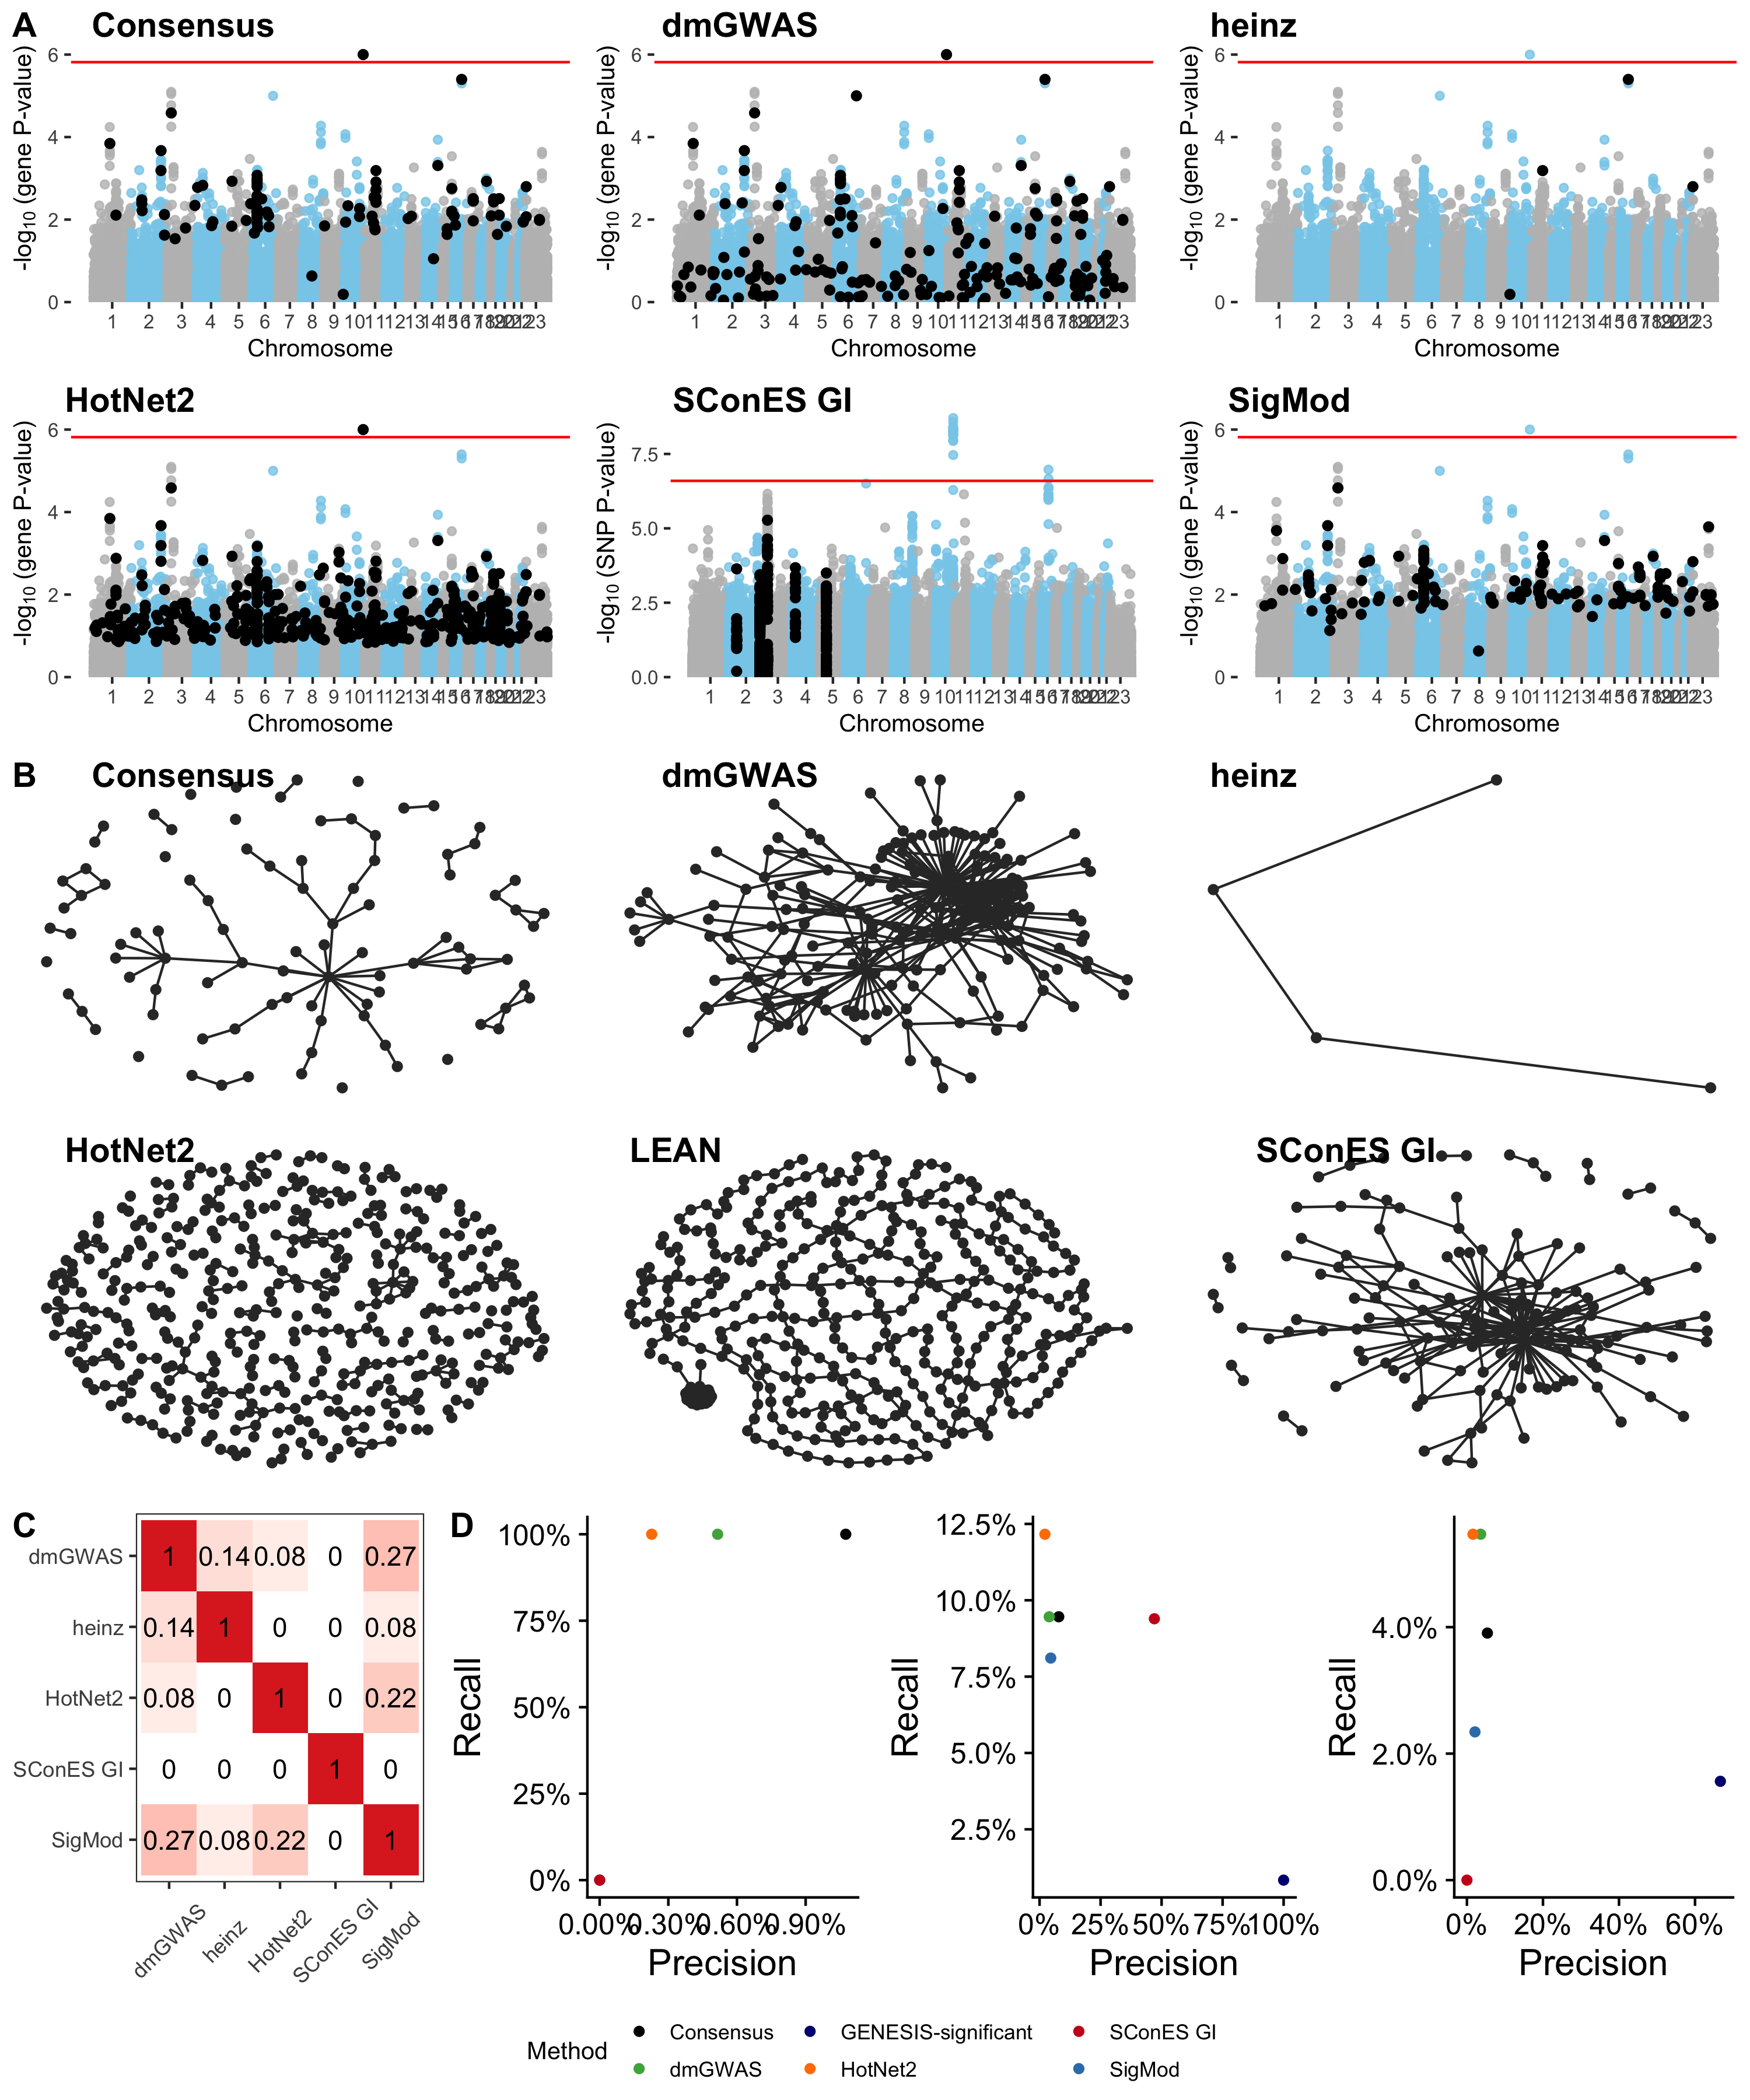
\includegraphics[width=.9\linewidth]{./figures/figure_1.png}
  \caption{\label{fig:solution_overview} TODO.}
\end{figure}

We applied six network methods to the GENESIS dataset (Section \ref{methods:methods}). As none of the networks examined by LEAN was significant (adjusted P-value < 0.05), we obtained five solutions (Supplementary Figure \ref{fig:solution_overview}, Supplementary Files 1 and 2): one for each of the remaining four gene-based methods (Section \ref{methods:gene_network}), and one for SConES GI (Section \ref{methods:snp_network}). The solutions are very heterogeneous (Table \ref{tab:gene_solutions} and Supplementary table \ref{tab:snp_solutions}), making hard to draw joint conclusions. HotNet2 produced the largest solution subnetwork with 440 genes. SConES GI failed to recover genes in the PPIN, but it recovered one genomic region mapped to RNA gene \emph{RNU6-420P}. All solution subnetworks except LEAN's have, on average, lower association P-values than the whole PPIN (median P-value $\ll 0.46$), despite containing genes with higher P-values (Supplementary Figure \ref{fig:solution_overview}A). This exemplifies the trade-off between statistical significance and biological relevance. However, there are nuances between solutions: heinz strongly favored high scoring genes, while dmGWAS is less conservative (median gene P-values 0.0012 and 0.19, respectively); SConES tended to select whole LD-blocks; and HotNet2 and SigMod were less likely to select low scoring genes. 

The solution subnetworks present other desirable properties. First, four of the methods succeeded at recovering known breast cancer susceptibility genes (Supplementary Figure \ref{fig:solution_overview}D), as their subnetworks were enriched in breast cancer susceptibility genes (dmGWAS, heinz, HotNet2, and SigMod, Fisher's exact test one-sided P-value < 0.03). We also compared the outcome of the network methods to the association tests conducted on the population of European ancestry from the Breast Cancer Association Consortium (BCAC) \cite{Michailidou2017} (Supplementary Figure \ref{fig:solution_overview}D). Encouragingly, every solution subnetwork is enriched in genes or SNPs that are Bonferroni-significant in BCAC. This confirms the capability of network methods to find the same signal as in more powered studies by leveraging on prior knowledge. Second, the genes in four solution subnetworks display on average a higher betweenness centrality than the rest of the genes, a difference that is significant in three solutions (dmGWAS, and SigMod, Wilcoxon rank-sum test P-value < 1.4 \texttimes{} 10\textsuperscript{-21}). This agrees with the notion that disease genes are more central than other, non-essential genes \cite{pinero_uncovering_2016}. We observe that this conclusion holds in this disease, as known breast cancer susceptibility genes have higher betweenness centrality than others (one-tailed Wilcoxon rank-sum test P-value = 2.64 \texttimes{} 10\textsuperscript{-5}, Supplementary Figure \ref{sfig:consensus_stats}C). Interestingly, SConES' selected SNPs are also more central than the average SNP (Supplementary table \ref{tab:snp_solutions}), suggesting that causal SNPs are also more central than unrelated SNPs. However, very central nodes are also more likely to be connecting a random pair of nodes, making then more likely to be selected by the examined methods. Hence, further work is needed draw conclusions.

As the solutions were quite different from each other it is hard to draw joint conclusions. The 4-gene solution selected by heinz includes the breast cancer susceptibility gene \emph{TOX3}, in region 16q12. By dealing with SNP networks, SConES studies the association of non-coding regions, as well as SNPs in any gene, coding or not. In fact, SConES GI, which adds to GM the interactions between genes, retrieves 4 subnetworks in intergenic regions, and 1 overlapping an RNA gene (\emph{RNU6-420P}). SigMod, despite being related to SConES, produces a vastly different, large solution. On top of recovering three breast cancer susceptibility genes, a keratin-based region of its subnetwork affects the cytoskeleton (\emph{structural constituent of cytoskeleton}, GO enrichment's adjusted P-value = 9.10 \texttimes{} 10\textsuperscript{-4}), a potentially novel susceptibility mechanism for cancer susceptibility. Interestingly, dmGWAS solution is also related to cytoskeleton (\emph{tubulin binding}, GO enrichment's adjusted P-value = 0.031). But, additionally, it includes a submodule of proteins related to \emph{unfolded protein binding} (GO enrichment's adjusted P-value = 0.045), which has been previously related to cancer susceptibility \cite{calderwood_heat_2016}. Lastly, HotNet2 produced 135 subnetworks, 115 of which have less than five genes. The second largest subnetwork (13 nodes), contains the two breast cancer susceptibility genes \emph{CASP8} and \emph{BLM}.

\subsection{A case study: the consensus network}
\label{results:consensus}
\begin{figure}[htbp]
  \centering
  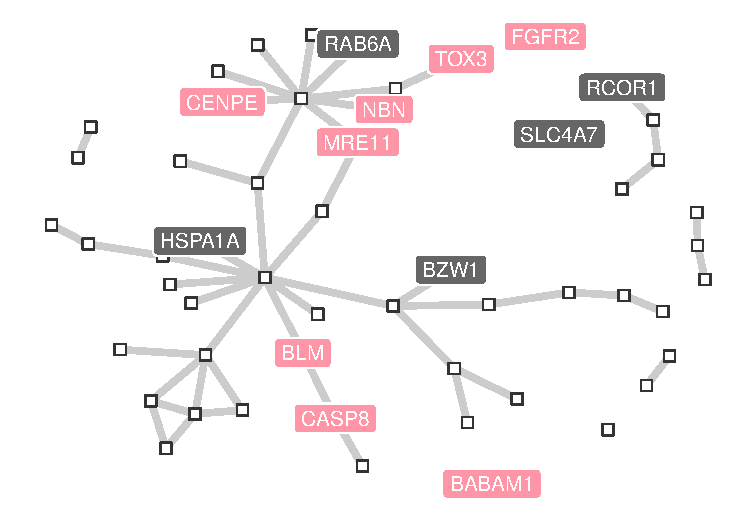
\includegraphics[width=.5\linewidth]{./figures/figure_3.pdf}
  \caption{\label{fig:consensus}
    Consensus subnetwork on GENESIS (Section \ref{methods:methods}). Each node is represented by a pie chart, which shows the methods that selected it. The labeled genes have a VEGAS2v2 P-value < 0.001 and/or are known breast cancer susceptibility genes (colored in pink).}
\end{figure}

The heterogeneity in the solutions suggested, and the shared encouraging properties suggested that each method was capturing different susceptibility mechanisms. Due to the limited overlap between methods, only 20 genes were common to more than two of them (Supplementary Figure \ref{sfig:consensus_stats}A). Encouragingly, the more methods selected a gene, the higher its association was (Supplementary Figure \ref{sfig:consensus_stats}B). To leverage on their strengths and compensate their respective weaknesses, we built a consensus subnetwork that captures the mechanisms most shared among the solution subnetworks (Section \ref{methods:methods}). This subnetwork (Figure \ref{fig:consensus}) contains 93 genes and shares the aforementioned properties of the individual solutions: enrichment in breast cancer susceptibility genes (Fisher's exact test P-value = 7.8 \texttimes{} 10\textsuperscript{-5}), higher betweenness centrality than the rest of the genes (Wilcoxon rank-sum test P-value = 4.29 \texttimes{} 10\textsuperscript{-18}) and TODO pathways. Topologically, the consensus network can be divided into a large connected component composed of 49 genes, and multiple smaller subnetworks. Among the latter, 14 of the 93 genes are in subnetworks containing a single gene or two connected nodes, implying that they do not have a consistently altered neighborhood, but are strongly associated themselves (TODO TEST). Some of them are known breast cancer susceptibility gene like \emph{FGFR2} (Section \ref{results:conventional}) and \emph{SLC4A7} (VEGAS P-value = 2.70 \texttimes{} 10\textsuperscript{-5}, \citet{ahmed_newly_2009}).

TODO Yet, there are other novel functions: Globally, a GO enrichment shows the involvement of two cellular processes: unfolded protein binding, and structural constituent of cytoskeleton (adjusted P-values of 0.001, 0.001, respectively), which were already observed in different solutions (Section \ref{results:separate_networks}). Remarkably, many of the selected genes are related to mitochondrial translation. For instance, MRPS30 (VEGAS P-value = 0.001), encodes a mitochondrial ribosomal protein and was also linked to breast cancer susceptibility \cite{quigley_5p12_2014}. Albeit disconnected from MRPS30, the consensus network includes a 2-node subnetwork composed of two mitochondrial ribosomal protein (MRPS31 - VEGAS P-value = 7.67 \texttimes{} 10\textsuperscript{-3} - and MRPS18B - VEGAS P-value = 7.92 \texttimes{} 10\textsuperscript{-3}), which suggests an involvement of mitochondrial ribosomes in carcinogenesis \cite{required}.

We also examined the topological properties of the nodes. The genes in the consensus network have higher betweenness centrality than the rest of the genes (Wilcoxon rank-sum test P-value = 4.29 \texttimes{} 10\textsuperscript{-18}). Interestingly, within genes in the consensus network, cancer genes are as central as non-cancer genes (Wilcoxon rank-sum test P-value = 0.57). The centrality in the PPIN of the genes in the consensus, however, is weakly anti-correlated with the P-value of association to the disease (Pearson correlation coefficient = -0.26, Supplementary Figure \ref{sfig:consensus_stats}D), which suggests that some highly central genes were selected because they were on the shortest path between two highly associated genes. In view of this, we hypothesize that highly central genes might contribute to the heritability through consistent alterations of their neighborhood, consistent with the omnigenic model of disease \cite{boyle_expanded_2017}. For instance, the most central node in the consensus network is \emph{COPS5} (Supplementary Figure \ref{sfig:consensus_names}), a gene related to multiple hallmarks of cancer and which is overexpressed in multiple tumors, including breast and ovarian cancer \cite{liu_jab1_cops5_2018}. Despite its lack of association in GENESIS (VEGAS P-value = 0.22), its neighbors in the consensus subnetwork have consistently low P-values (median VEGAS P-value = 0.006).

% The consensus subnetwork is not completely connected: out of the 93 genes, the largest connected subnetwork includes only 49. A GO enrichment analysis showed that this component is related to three major cellular processes: unfolded protein binding, structural constituent of cytoskeleton, and poly(U) RNA binding (adjusted P-values of 0.01, 0.04, and 0.04, respectively). We found support in the literature of the involvement of each of these functions in the development of cancer, as discussed next. The consensus network also contains a protein directly involved in caspase-mediated apoptosis, \emph{CASP8} (VEGAS P-value = 1.95 \texttimes{} 10\textsuperscript{-4}). This is related to the enriched activity, \emph{unfolded protein binding}, which inhibits caspase-dependent apoptosis, raising the chances of developing cancer \cite{calderwood_heat_2016}. It involves three Hsp70 chaperones of the consensus subnetwork: HSPA1A, HSPA1B, and HSPA1L. The genes encoding these proteins are all near each other at 6p21. In fact, out of the 22 SNPs that map to any of these three genes, 9 map to all of them, and 4 to two, making hard to disentangle their association. \emph{HSPA1A} was the most strongly associated one (VEGAS P-value = 8.37 \texttimes{} 10\textsuperscript{-4}). 

\subsection{Methods are comparably stable, and produce similarly good predictors}

\begin{figure}[htbp]
\centering
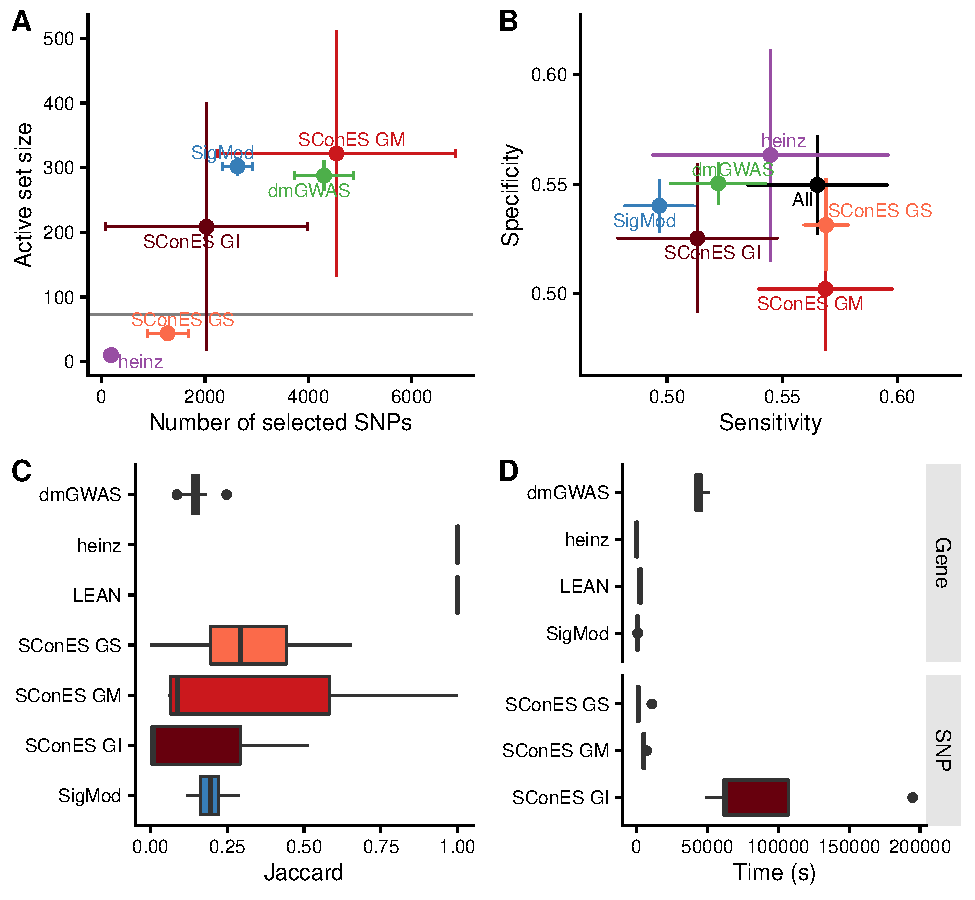
\includegraphics[width=.8\linewidth]{./figures/figure_4.pdf}
\caption{\label{fig:benchmark}
Comparison of network-based GWAS methods on GENESIS. Each method was run 5 times of a random subset of the samples, and tested on the remaining samples (Sections \ref{methods:comparison} and \ref{methods:classifier}). \textbf{(A)} Number of SNPs selected by each method and number of SNPs on the active set used by the Lasso classifier. Points are the average over the 5 runs; lines represent the standard error of the mean. A grey diagonal line with slope 1 is added for comparison. For reference, the active set of Lasso using all the SNPs included, on average, 154\,117.4 SNPs. \textbf{(B)} Sensitivity and specificity on test set of the L1-penalized logistic regression trained on the features selected by each of the methods. In addition, the performance of the classifier trained on all SNPs is displayed. Points are the average over the 5 runs; lines represent the standard error of the mean. \textbf{(C)} Pairwise Pearson's correlations of the solutions used by different methods. A Pearson's correlation of 1 means the two solutions are the same. A Pearson's correlation of 0 means that there is no SNP in common between the two solutions. \textbf{(D)} Runtime of the evaluated methods, by type of network used (gene or SNP). For gene network-based methods, inverted triangles represent the runtime of the algorithm itself, and circles the total time, which includes the algorithm themselves and the additional 119\,980 seconds (1 day and 9.33 hours) which took VEGAS2v2 on average to compute the gene scores from SNP summary statistics.}
\end{figure}

We compared the six methods in a 5-fold subsampling setting (Sections \ref{methods:comparison} and \ref{methods:classifier}). Specifically, we measured five properties (Figure \ref{fig:benchmark}): size of the solution subnetwork; sensitivity and specificity of an L1-penalized logistic regression classifier on the selected SNPs; stability; and computational runtime.

Both solution size and the subset of it selected by the classifier (\emph{active set}) varies greatly between the different methods (Figure \ref{fig:benchmark}A). Heinz produced the smallest solutions, with an average of 182 selected SNPs. The largest solutions come from SConES GI (6\,256.6 SNPs), and dmGWAS (4\,255.0 SNPs). Interestingly, heinz has the highest proportion of the selected SNPs that go into the active set (99.9\%), although it is  high for all the methods (> 86\%). To determine whether the selected SNPs could be used for patient classification we computed the performance of the classifier on the \emph{test dataset} (Figure \ref{fig:benchmark}B). The different classifiers displayed similar sensitivities and specificities, all in the 0.52 -- 0.56 range.

Another desirable quality of an algorithm is stability of the solution with regards to different inputs (Section \ref{methods:comparison}). Both heinz and LEAN displayed a high stability in our benchmark, consistently selecting the same genes and no genes over the 5 subsamples, respectively (Figure \ref{fig:benchmark}C). Conversely, the other methods displayed similarly low stabilities. 

In terms of computational runtime, the fastest method was heinz (Figure \ref{fig:benchmark}D), which leverages on its ability to find efficiently the solution in a few seconds, and HotNet2 was slowest (3 days and 14 hours on average). Including the time required to compute the gene scores slows down considerably gene-based methods; on this benchmark, that step took on average 1 day and 9.33 hours. Considering that, it took 5 days on average for HotNet2 to produce results. 

\subsection{The consensus overcomes the problems of the individual solutions}
\label{results:drawbacks}

\begin{figure}[htbp]
\centering
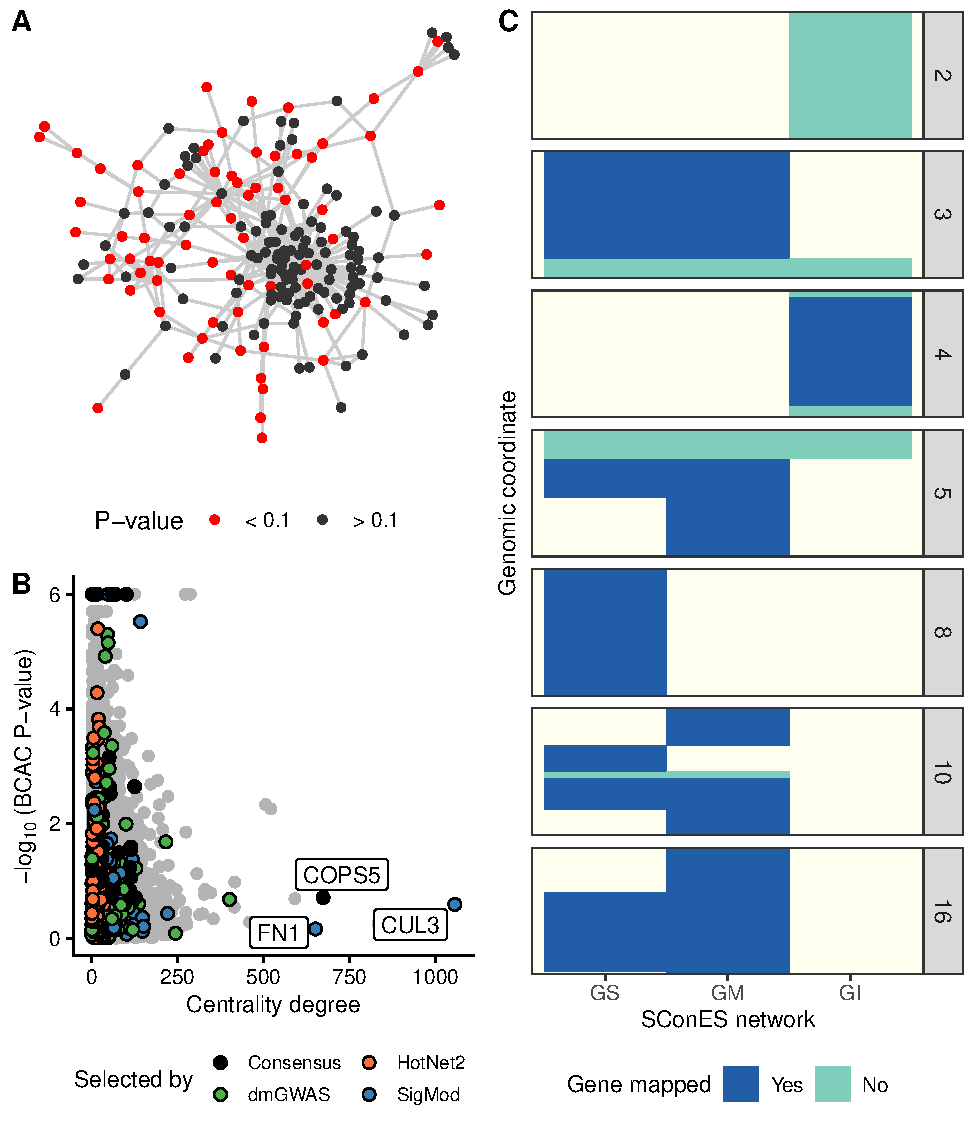
\includegraphics[width=.8\linewidth]{./figures/figure_2.pdf}
\caption{\label{fig:issues}
Drawbacks confronted when using network guided methods. \textbf{(A)} dmGWAS solution subnetwork. Genes with a P-value < 0.1 are highlighted in red. \textbf{(B)} Centrality degree and -log\textsubscript{10} of the VEGAS2v2 P-value for the nodes in SigMod solution subnetwork. \textbf{(C)} Genomic regions where either SConES GS, GM or GI select SNPs.}
\end{figure}

In practice, and despite their similarities and their involvement in cancer mechanisms, the solutions are remarkably different (Supplementary Figure \ref{sfig:pearson_methods}A). That is due to the particularities of the methods which directly or indirectly provide information about the dataset. For instance, the fact that LEAN did not provide any biomarkers implies that there is no gene such that both itself and its environment are on average strongly associated with the disease. 

In this dataset, heinz's solution is very conservative, providing a small solution with the lowest median P-value for the subnetwork (Table \ref{tab:gene_solutions}). Due to this parsimonious and highly associated solution, it was the best method to select a set of good biomarkers for classification. (Figure \ref{fig:benchmark}B). Its conservativeness stems from its preprocessing step, which models the gene P-values as a mixture model of a beta and a uniform distribution, controlled by an FDR parameter. Due to the limited signal at the gene level in this dataset (Figure \ref{sfig:snp_gene_manhattan}B), only 36 of them are retain a positive score after applying the BUM model (Section \ref{methods:methods}). Hence, heinz's solution subnetwork consists only of 4 genes, which does not provide much insight of the biology of cancer. Importantly, it ignores genes that are associated to cancer in this dataset like \emph{FGFR2}. 

On the other end of the spectrum, we have large solutions provided by dmGWAS, HotNet2, and SigMod. dmGWAS' subnetwork is the least associated subnetwork on average. This is due to the greedy framework it uses, which has a bias for larger solutions \cite{nikolayeva_network_2018}. This framework considers all nodes at distance 2 of the examined, and accepts weakly associated genes if they are linked to another, strongly associated one. This is exacerbated when the results of successive greedy searches are aggregated, leading to a large, tightly connected cluster of unassociated genes (Figure \ref{fig:issues}A). SigMod displays the same tendency, as the most central genes are the least associated to the disease (Figure \ref{fig:issues}B). This relatively low signal-to-noise ratio combined with the large solution requires additional analyses to draw conclusions, such as enrichment analyses. In the same line, HotNet2's subnetwork is even harder to interpret, being composed of 440 genes divided into 135 subnetworks. Lastly, SigMod misses some of the most strongly associated, breast cancer susceptibility genes in the dataset, like \emph{FGFR2} and \emph{TOX3}.

By virtue of using a SNP subnetwork, SConES analyzes each SNP in their context. It therefore selects SNPs in genes none of whose interactors are associated to the disease, as well as SNPs in non-coding regions or in non-interacting genes. In fact, due to linkage disequilibrium, such genes are favored by SConES, as selecting SNPs in an LD block which overlaps with a gene favors selecting the rest of the gene. This might explain why the GS and GM networks, heavily affected by linkage disequilibrium, produce similar results (Supplementary Figure \ref{sfig:pearson_methods}B). On the other hand, SConES penalizes selecting SNPs and not their neighbors. This makes it conservative regarding SNPs with many interactions, for instance those mapped to hubs in the PPIN. For this reason, SConES GI did not select any protein coding gene, despite selecting similar regions as SConES GS (Figure \ref{fig:issues}C). In fact SConES GS and SConES GM select regions related to breast cancer, like 16q12 (\emph{TOX3}, Section \ref{results:conventional}), 3p24 (\emph{SLC4A7}/\emph{NEK10} \cite{ahmed_newly_2009}), 5p12 (\emph{FGF10}, \emph{MRPS30} \cite{quigley_5p12_2014}), and 10q26 (\emph{FGFR2}, Section \ref{results:conventional}). On top of that only SConES GS selects region 8q24 (\emph{POU5F1B} \cite{breyer_expressed_2014}). We hypothesize that the lack of results on the PPIN network of SConES GI and LEAN are due to the same cause: the absence of joint association of a module. Although in the case of SConES other hyperparameters could lead to a more informative solution (e.g. lower \(\lambda\), Section \ref{methods:methods}), it is unclear what is the best strategy to find them. In addition, due to the iCOGS SNP array design, the genome of GENESIS participants has not been unbiasedly surveyed: some regions are fine-mapped --- which might distort gene structure in GM and GI networks --- while others are under studied --- hurting the accuracy with which the GS network captures the genome structure.

\subsection{Network methods boost biomarker discovery}

We compared the results of different network methods to the European cohort of BCAC, the largest GWAS to date in breast cancer (Section \ref{methods:bcac}). This comparison is pertinent, since despite caveats we expect a significant shared genetic factors with GENESIS, and since it is a much larger study (XX times more samples, 13 million SNPs through imputation). We conducted a study at both the SNP and the gene levels, equivalent to the one shown in Section \ref{results:conventional} for GENESIS. Despite the low overlap using a conventional approach (TODO), the solutions provided by the different network approaches overlap significantly (Fisher's exact test P-value $\leq X \times 10^{-X}$). This illustrates the ability of network guided GWAS to boost discovery.

\section{Discussion}

In this article we evaluate the viability of a systems biology take on genetic studies by examining a GWAS dataset on familial breast cancer. Such an approach addresses two of the largest issues with GWAS: interpretability and an overly conservative statistical framework that hinders discovery. This is achieved by considering the biological context of each of the genes and SNPs. Based on divergent considerations of what the desired set of biomarkers is, several methods for network-guided biomarker discovery have been proposed. We reviewed the performance of six of them on GWAS. Despite their differences, most of them produced a relevant subset of biomarkers, recovering known familial breast cancer genes. We also discuss the limitations of such analyses, related to the lack of known interactions around some genes. 

A crucial step for the gene based methods is the computation of the gene score. In this work we used VEGAS2v2 \cite{mishra_vegas2:_2015} due to the flexibility it offers to use user-specified gene annotations. However, it presents known problems (selection of an appropriate percentage of top SNPs, long runtimes and P-value precision limited to the number of permutations \cite{nakka_gene_2016}), and other algorithms might have more statistical power. Another important decision is how to handle LD in a GWAS. VEGAS2v2 accounts for LD patterns, and hence an LD pruning step would not impact gene-based network methods, although it would speed up VEGAS2v2's computation time. With regards to SConES, less SNPs would lead to simpler SNP networks and, possibly, shorter runtimes. However, as mentioned in Section \ref{results:drawbacks}, LD patterns seem paramount to SConES' solutions, and an LD pruning step could potentially alter them. 

The network methods we studied differ in what the optimal solution subnetwork looks like, which acted as a double-edged sword. In one end of the spectrum, SConES and heinz preferred small, highly associated solutions, providing a conveniently short list of biomarkers, at the expense of not shedding much light on the etiology of the disease. On the other end, SigMod and dmGWAS gravitate towards larger, less associated solutions which provide a wide overview of the biological context. While this deepens our understanding of the disease and provide biological hypotheses, they require further analyses, which risk oversimplifying their richness. HotNet2 balances both approaches at the expense of producing a constellation of many, highly associated, small subnetworks. Despite their differences, all the solutions produced comparable discrimination capabilities on a linear classifier trained on them. On the negative side, the methods were also remarkably unstable, and hence likely to produce very different solutions in face of slightly different inputs.

To overcome the problems posed by the individual methods while exploiting their strengths, we propose combining them into a consensus subnetwork. We use a straightforward aggregation to generate it, including any node that was recovered by at least two methods. The resulting network is a synthesis of the altered mechanism: it is smaller than the largest solutions (SigMod and dmGWAS), which makes it more manageable, and includes the majority of the strongly associated smaller solutions (SConES and heinz). The consensus subnetwork captures mechanisms and genes known to be related to cancer, recovering known breast cancer susceptibility genes as well as genome regions associated to breast cancer susceptibility. However, thanks to its smaller size and its network structure, it provides compelling hypotheses of non-canonical mechanisms involved in carcinogenesis, like mitochondrial translation and chaperone activity.

The strength of network-based analyses comes from leveraging prior knowledge to boost discovery. In consequence, they show their shortcomings in front of understudied genes, especially those not in the network. Out of the 32\,767 genes that we can map the genotyped SNPs to, 60.7\% (19\,887) are not in the protein-protein interaction network. The majority of those (14\,660) are non-coding genes, mainly lncRNA, miRNA, and snRNA (Supplementary Figure \ref{sfig:biotypes_excluded}). Yet, RNA genes like \emph{CASC16} are associated to breast cancer (Section \ref{results:conventional}), reminding us of the importance of using networks beyond coding genes. Even protein-coding genes linked to breast cancer susceptibility \cite{ahmed_newly_2009}, like \emph{NEK10} (P-value 1.6 \texttimes{} 10\textsuperscript{-5}, located near \emph{SLC4A7}) or \emph{POU5F1B}, were absent from the network. However, on average protein-coding genes absent from the PPIN are less associated with this phenotype (Wilcoxon rank-sum P-value = 2.79 \texttimes{} 10\textsuperscript{-8}, median P-values of 0.43 and 0.47). As we are using interactions from high-throughput experiments, such difference cannot be due to well-known genes having more known interactions. As disease genes tend to be more central \cite{pinero_uncovering_2016}, we hypothesize that it is due to interactions between central genes being more likely. It is worth noting that network approaches that do not use PPIs, like SConES GS and GM, did recover SNPs in \emph{NEK10} and \emph{CASC16}. This shows the potential of SNP networks, in which SNPs are linked when there is evidence of co-function, to perform network-guided GWAS even in the absence of gene-level interactions. Lastly, all the methods rely heavily on how SNPs are mapped to genes. In Section \ref{results:conventional} we highlight ambiguities that appear when genes overlap or are in linkage disequilibrium.

As not all databases compile the same interactions, the choice of the PPIN determines the final output. In this work we used exclusively interactions from HINT from high-throughput experiments. This responds to concerns of some authors about adding interactions identified in targeted studies and prone to a ``rich getting richer'' phenomenon: popular genes have a higher proportion of their interactions described \cite{cai_broker_2010,das_hint:_2012}. Their presense might bias the results of the presented methods, as if changes the topology of the networks by adding nodes closer on average to other nodes than average. On the other hand, \citet{huang_systematic_2018} found that the best predictor of the performance of a network for disease gene discovery is the size of the network, which supports using the largest amount of interactions. When we compared the impact of using a larger network containing interactions from both high-throughput experiment and the literature (Section \ref{methods:gene_network}), we found that for most of the methods it did not greatly change the size or the stability of the solution, the classification accuracy, or the runtime (Supplementary Figure \ref{sfig:lc_ht_comparison}). This supports using only interactions from high-throughput experiments, which produces apparently similar solutions and avoids falling into ``circular reasonings'', where the best known genes are artificially pushed into the selected solutions. 

In order to produce the consensus network, we had to face the different interfaces, preprocessing steps, and unexpected behaviors of the various methods. To facilitate that other authors apply them to new datasets and aggregate their solutions, we built six nextflow pipelines \cite{di_tommaso_nextflow_2017} with a consistent interface and, whenever possible, parallelized computation. They are available on GitHub: \url{https://github.com/hclimente/gwas-tools}. Importantly, those methods that had a permissive license were compiled into a Docker image for easier use, which is available on Docker Hub \href{https://hub.docker.com/r/hclimente/gwas-tools}{hclimente/gwas-tools}.

\section*{Author contributions}

H.C-G. conducted all the final analyses and the writing of the manuscript. C.L. conducted analyses using LEAN, Sigmod, and dmGWAS, and provided help and feedback. F.L. and N.A. provided feedback on the analyses and the manuscript. C-A.A. supervised the project.

\section*{Funding and acknowledgments}

This project was supported by funding from Agence Nationale de la Recherche (ANR-18-CE45-0021-01) and from the European Union’s Horizon 2020 research and innovation program (Marie Skłodowska-Curie [666003]). Financial support for GENESIS resource and genotyping was provided by the Ligue Nationale contre le Cancer (grants PRE05/DSL, PRE07/DSL, PRE11/NA), the French National Institute of Cancer (INCa grant b2008-029/LL-LC) and the comprehensive cancer center SiRIC (Site de Recherche Intégrée sur le Cancer: INCa-DGOS-4654).

We wish to thank the genetic epidemiology platform (the PIGE, Plateforme d'Investigation en Génétique et Epidemiologie: O. Kulkarni, S. Eon-Marchais, M. Marcou, D. Le Gal, L. Toulemonde, J. Beauvallet, N. Mebirouk, E. Cavaciuti), the biological resource centre (S. Mazoyer, F. Damiola, L. Barjhoux, C. Verny-Pierre, V. Sornin) and all the GENESIS collaborating cancer clinics clinics (Clinique Sainte Catherine, Avignon: H. Dreyfus; Hôpital Saint Jacques, Besançon: M-A. Collonge-Rame; Institut Bergonié, Bordeaux: M.Longy, A. Floquet, E. Barouk-Simonet; CHU, Brest: S. Audebert; Centre François Baclesse, Caen: P. Berthet; Hôpital Dieu, Chambéry: S. Fert-Ferrer; Centre Jean Perrin, Clermont-Ferrand: Y-J. Bignon; Hôpital Pasteur, Colmar: J-M. Limacher; Hôpital d’Enfants CHU – Centre Georges François Leclerc, Dijon: L. Faivre-Olivier; CHU, Fort de France: O. Bera; CHU Albert Michallon, Grenoble: D. Leroux; Hôpital Flaubert, Le Havre: V. Layet; Centre Oscar Lambret, Lille: P. Vennin, C. Adenis; Hôpital Jeanne de Flandre, Lille: S. Lejeune-Dumoulin, S. Manouvier-Hanu; CHRU Dupuytren, Limoges: L. Venat-Bouvet; Centre Léon Bérard, Lyon: C. Lasset, V. Bonadona; Hôpital Edouard Herriot, Lyon: S. Giraud; Institut Paoli-Calmettes, Marseille: F. Eisinger, L. Huiart; Centre Val d’Aurelle – Paul Lamarque, Montpellier: I. Coupier; CHU Arnaud de Villeneuve, Montpellier: I. Coupier, P. Pujol; Centre René Gauducheau, Nantes: C. Delnatte; Centre Catherine de Sienne, Nantes: A. Lortholary; Centre Antoine Lacassagne, Nice: M. Frénay, V. Mari; Hôpital Caremeau, Nîmes: J. Chiesa; Réseau Oncogénétique Poitou Charente, Niort: P. Gesta; Institut Curie, Paris: D. Stoppa-Lyonnet, M. Gauthier-Villars, B. Buecher, A. de Pauw, C. Abadie, M. Belotti; Hôpital Saint-Louis, Paris: O. Cohen-Haguenauer; Centre Viggo-Petersen, Paris: F. Cornélis; Hôpital Tenon, Paris: A. Fajac; GH Pitié Salpétrière et Hôpital Beaujon, Paris: C. Colas, F. Soubrier, P. Hammel, A. Fajac; Institut Jean Godinot, Reims: C. Penet, T. D. Nguyen; Polyclinique Courlancy, Reims: L. Demange, C. Penet; Centre Eugène Marquis, Rennes: C. Dugast; Centre Henri Becquerel, Rouen: A. Chevrier, T. Frebourg, J. Tinat, I. Tennevet, A. Rossi; Hôpital René Huguenin/Institut Curie, Saint Cloud: C. Noguès, L. Demange, E. Mouret-Fourme; CHU, Saint-Etienne: F. Prieur; Centre Paul Strauss, Strasbourg: J-P. Fricker, H. Schuster; Hôpital Civil, Strasbourg: O. Caron, C. Maugard; Institut Claudius Regaud, Toulouse: L. Gladieff, V. Feillel; Hôpital Bretonneau, Tours: I. Mortemousque; Centre Alexis Vautrin, Vandoeuvre-les-Nancy: E. Luporsi; Hôpital de Bravois, Vandoeuvre-les-Nancy: P. Jonveaux; Gustave Roussy, Villejuif: A. Chompret, O. Caron). 

\bibliographystyle{abbrvnat}
\bibliography{bibliography}

\clearpage
\setcounter{figure}{0}
\setcounter{section}{0}
\setcounter{table}{0}

\section*{Supplementary materials}

\begin{table}[htbp]
\begin{threeparttable}
\caption{\label{tab:snp_solutions}
Summary statistics on the results of SConES on the three SNP-SNP interaction networks. The first row within each block contains the summary statistics on the whole network.}
\centering
\begin{tabular}{lrrllr}
Network & SNPs & Edges & Subnetworks & \mean{Betweenness} & \median{P}\textsubscript{SNP}\\
\hline
GS & 197\,083 & 197\,060 & - & 2.03 \texttimes{} 10\textsuperscript{7} & 0.49\\
SConES GS & 1\,590 & 1\,585 & 5 & 2.52 \texttimes{} 10\textsuperscript{7} & 0.023\\
\hline
GM & 197\,083 & 6\,442\,446 & - & 3.99 \texttimes{} 10\textsuperscript{6} & 0.49\\
SConES GM & 1\,692 & 177\,611 & 5 & 4.40 \texttimes{} 10\textsuperscript{6} & 0.055\\
\hline
GI & 197\,083 & 28\,733\,720 & - & 1.46 \texttimes{} 10\textsuperscript{6} & 0.49\\
SConES GI & 408 & 539 & 5 & 9.33 \texttimes{} 10\textsuperscript{6} & 0.076\\
\end{tabular}
\begin{tablenotes}
\item \mean{Betweenness}: mean betweenness of the selected SNPs in the corresponding full network.
\item \median{P}\textsubscript{SNP}: median P-value of the selected SNPs.
\end{tablenotes}
\end{threeparttable}
\end{table}

\begin{table}[htbp]
\begin{threeparttable}
  \caption{\label{tab:scones_gene_solutions}
Summary statistics on the results of multiple network methods on the gene-gene interaction network. The first row contains the summary statistics on the whole network.}
\centering
\begin{tabular}{lrrrlr}
Network & Genes & Edges & \mean{Betweenness} & \median{P}\textsubscript{gene} & $\rho_{consensus}$\\
\hline
SConES GS & 5 & 0 & 9\,805 & 2.7 \texttimes{} 10\textsuperscript{-5} & 0.19\\
SConES GM & 28 & 2 & 4\,267 & 0.067 & 0.12\\
\end{tabular}
\begin{tablenotes}
\item \mean{Betweenness}: mean betweenness of the selected genes in the full network.
\item \median{P}\textsubscript{gene}: median P-value of the selected genes; $\rho_{consensus}$: Pearson's correlation with the consensus network.
\end{tablenotes}
\end{threeparttable}
\end{table}

\begin{figure}[htbp]
\centering
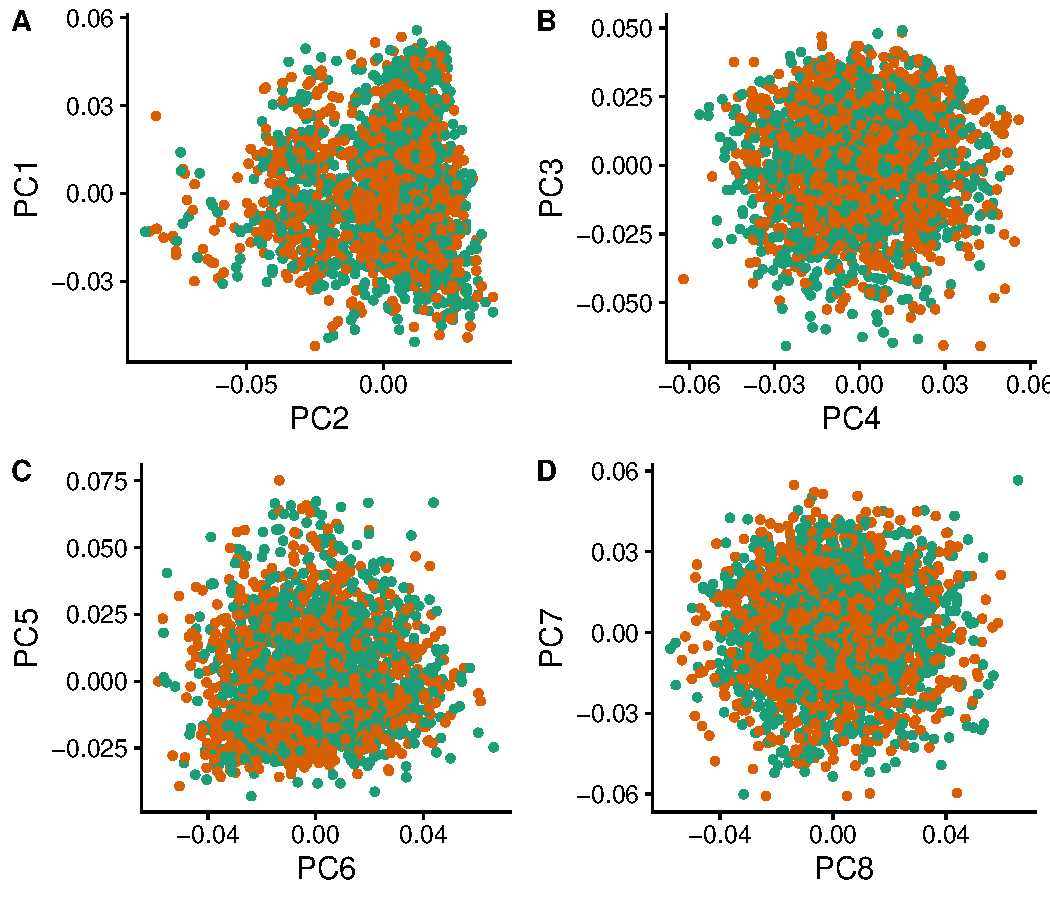
\includegraphics[width=.9\linewidth]{./figures/sfigure_1.pdf}
\caption{\label{sfig:pcs} GENESIS shows no differential population structure between cases and controls. \textbf{(A,B,C,D)} Eight main principal components computed on the genotypes of GENESIS. Cases are colored in green, controls in orange.}
\end{figure}

\begin{figure}[htbp]
  \centering
  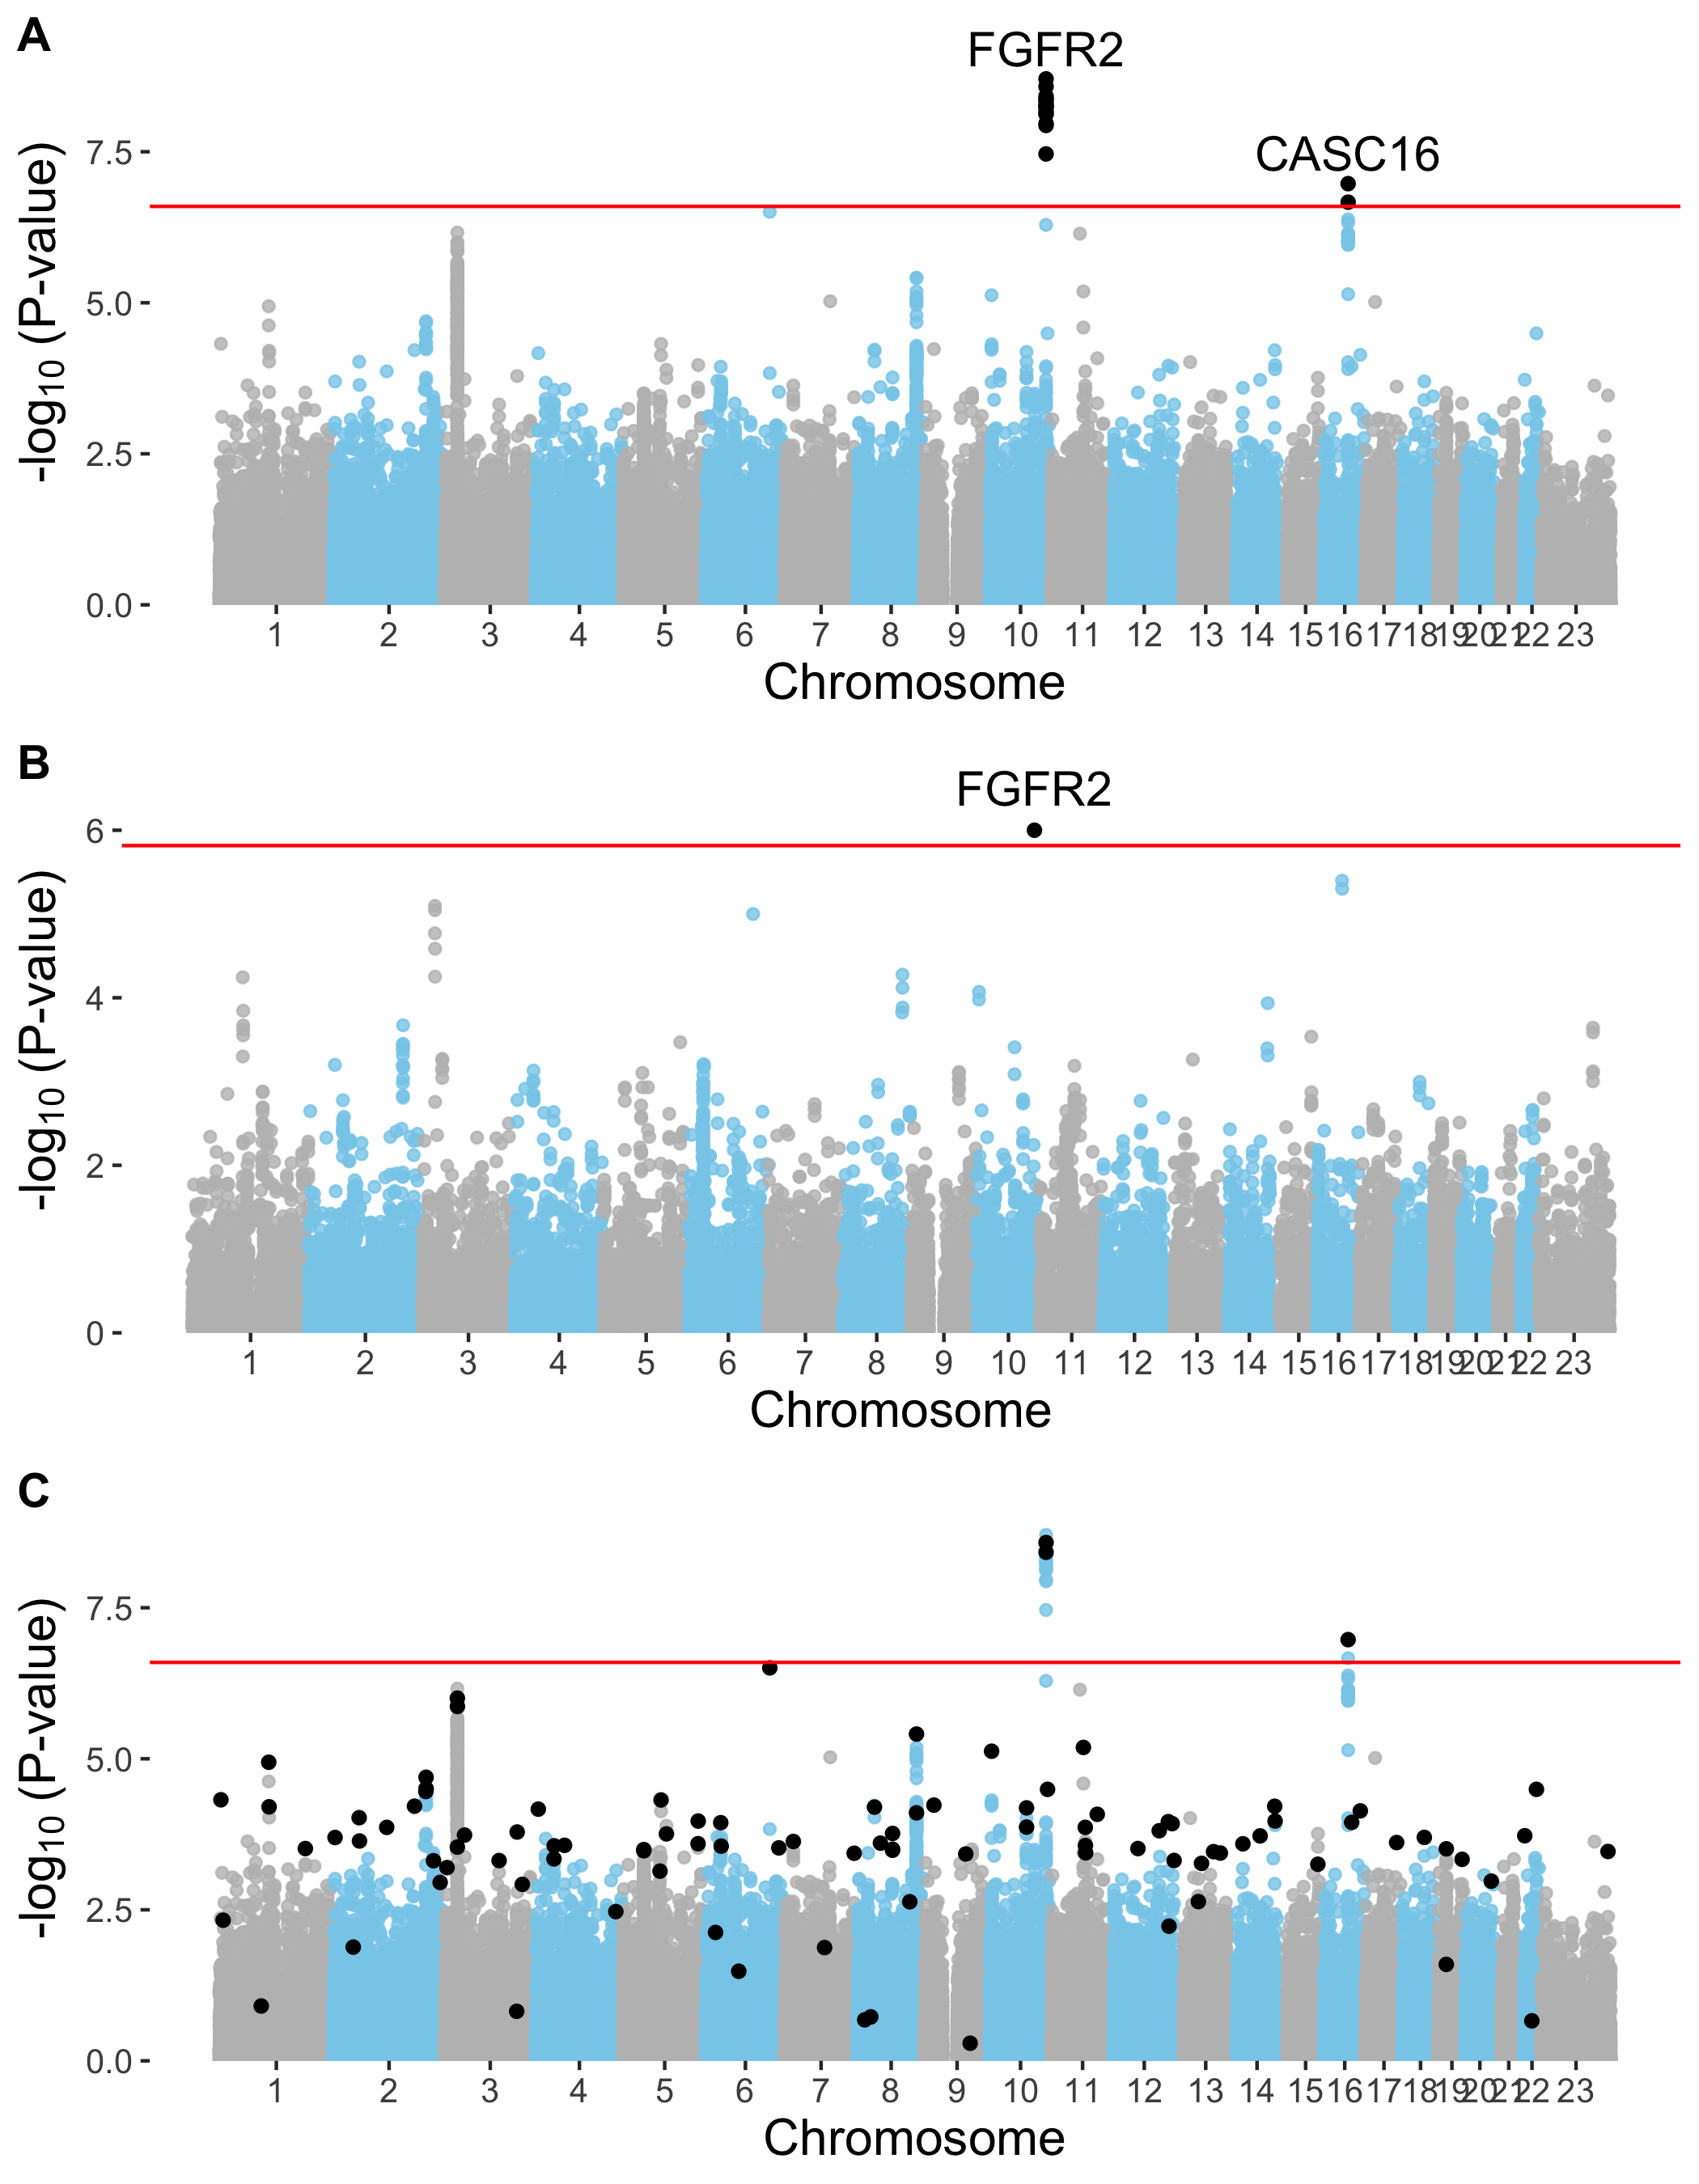
\includegraphics[width=.9\linewidth]{./figures/sfigure_2.png}
  \caption{\label{sfig:snp_gene_manhattan} Association in GENESIS. The red line represents the Bonferroni threshold. \textbf{(A)} SNP association, measured from the outcome of a 1 d.f. $\chi^2$ allelic test. Significant SNPs that are within a coding gene, or within 50 kilobases of its boundaries, are annotated. The Bonferroni threshold is 2.54 \texttimes{} 10\textsuperscript{-7}. \textbf{(B)} Gene association, measured by P-value of VEGAS2v2 \cite{mishra_vegas2:_2015} using the 10\% of SNPs with the lowest P-values. The Bonferroni threshold is 1.53 \texttimes{} 10\textsuperscript{-6}. \textbf{(C)} SNP association as in panel (A). The SNPs in black are selected by a L1-penalized logistic regression (Section \ref{methods:classifier}, $\lambda = 0.03$).}
\end{figure}

\begin{figure}[htbp]
\centering
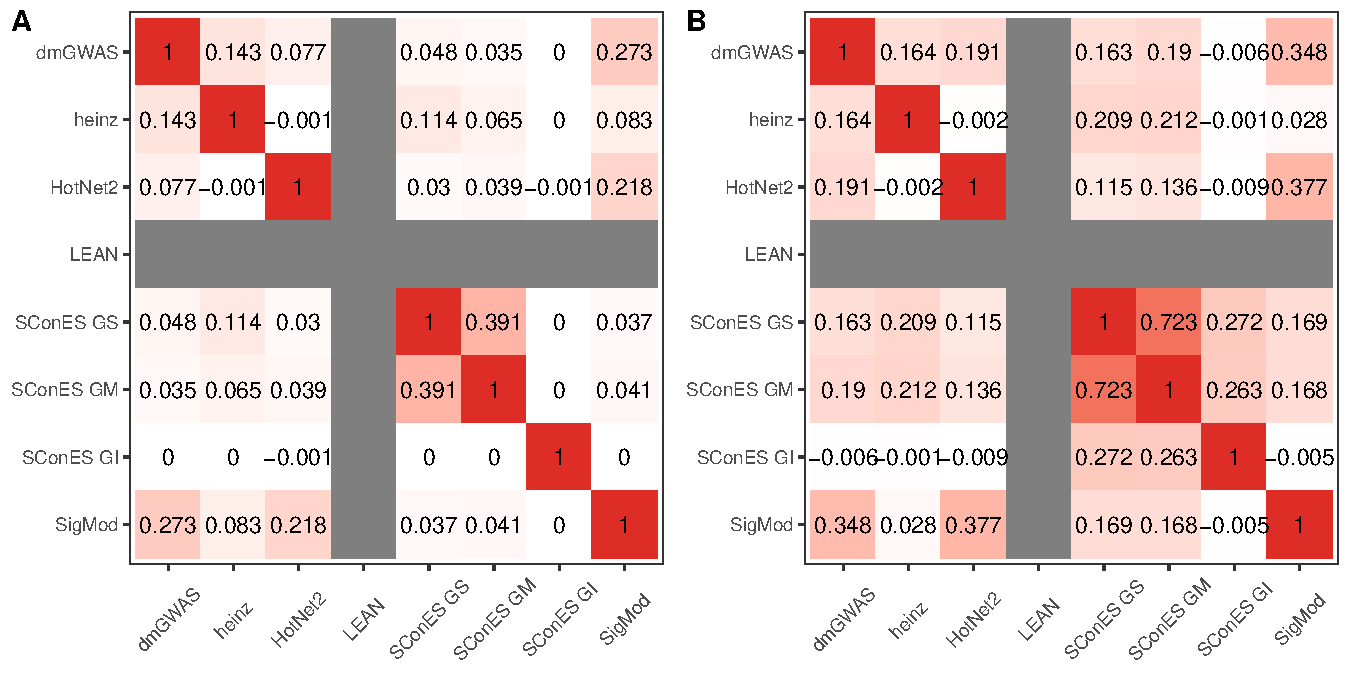
\includegraphics[width=.9\linewidth]{./figures/sfigure_3.pdf}
\caption{\label{sfig:pearson_methods}
Pearson's correlation between the different solution subnetworks. \textbf{(A)} Correlation between selected SNPs. \textbf{(B)} Correlation between selected genes. In general, the solutions display a very low overlap.}
\end{figure}

\begin{figure}[htbp]
\centering
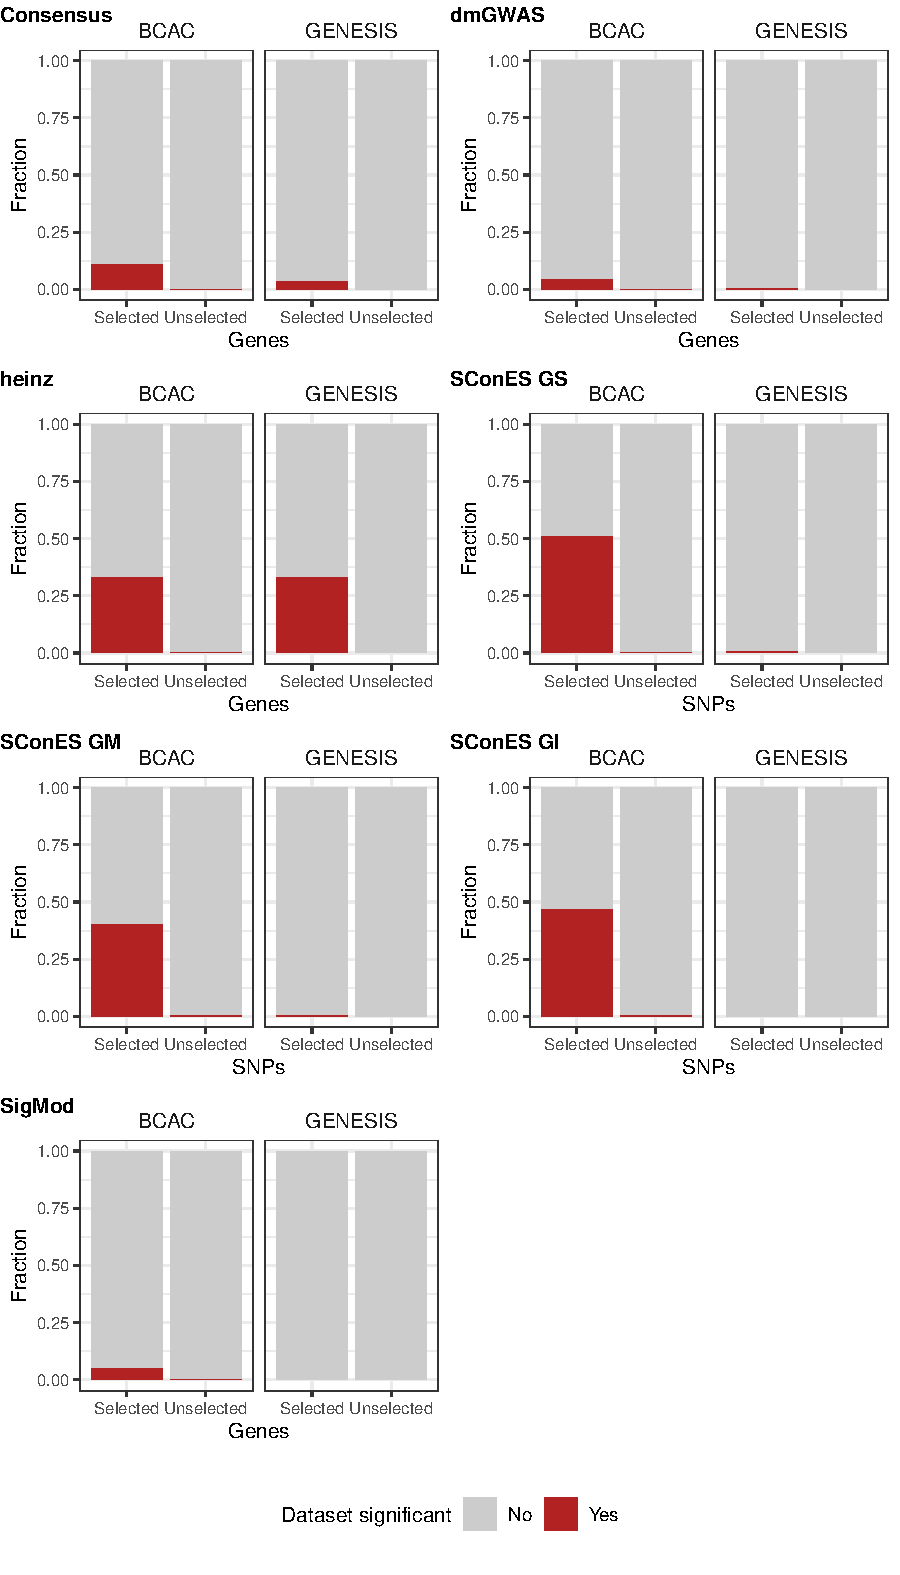
\includegraphics[width=.9\linewidth]{./figures/sfigure_4.pdf}
\caption{\label{sfig:consensus_names}
Consensus subnetwork on GENESIS (Section \ref{methods:methods}). \textbf{(A)} Each node is represented by a pie chart, which shows the methods that selected it. The labeled genes have a VEGAS2v2 P-value < 0.001 and/or are known breast cancer susceptibility genes (colored in pink). This panel is identical to Figure \ref{fig:consensus}. \textbf{(B)} Manhattan plot showing the genes included in the subnetwork. \textbf{(C)} Every gene name is indicated. \textbf{(D,E)} Proportion of the Bonferroni significant genes (in GENESIS and BCAC, respectively) included in the consensus network. \textbf{F} Proportion of the selected genes by each of the methods on the GENESIS data that is a known breast cancer susceptibility gene, as in Figure \ref{fig:solution_overview}D}.
\end{figure}

\begin{figure}[htbp]
\centering
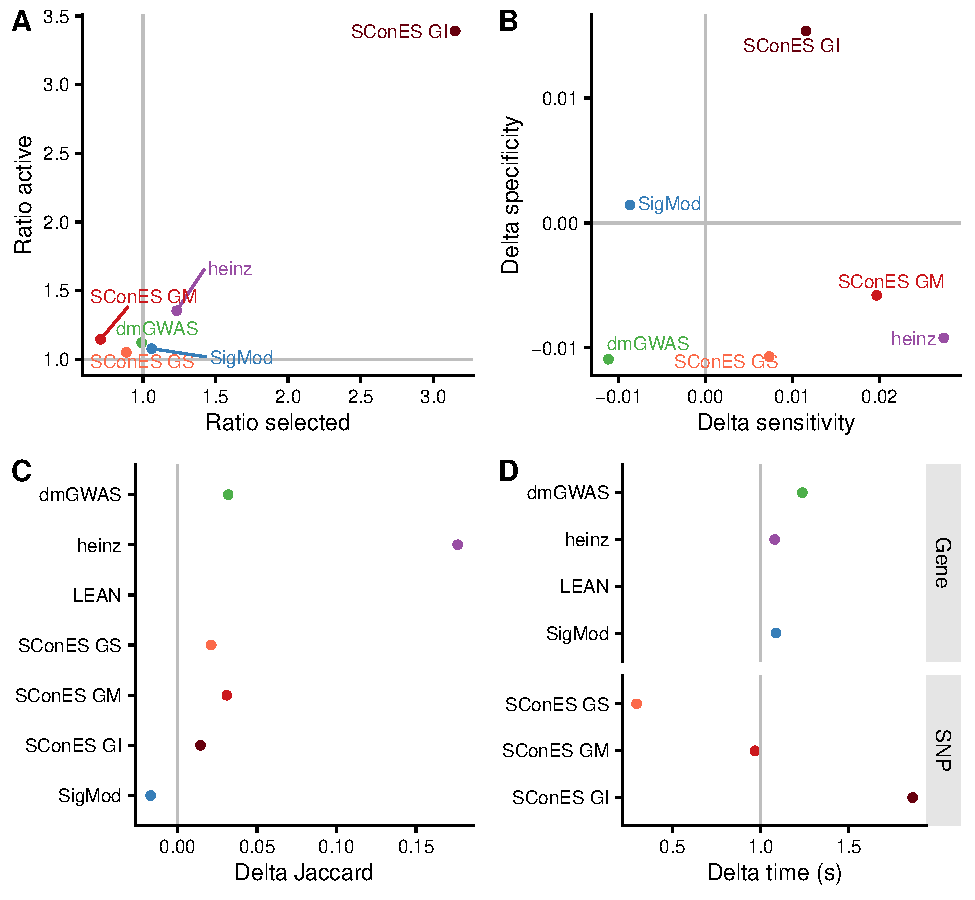
\includegraphics[width=\textwidth,height=\textheight,keepaspectratio]{./figures/sfigure_5.pdf}
\caption{\label{sfig:consensus_stats}
Genes on the consensus network. Breast cancer susceptibility genes are colored in pink; the rest are colored in grey. \textbf{(A)} Number of methods selecting every gene in the subnetwork. \textbf{(B)} VEGAS P-values of association of the genes, with regards to the number of methods that selected them. \textbf{(C)} Comparison of betweenness centrality of the genes in the consensus network and the other genes in the PPIN and not in the consensus network. To improve visualization, we removed outliers. \textbf{(D)} Relationship between the log\textsubscript{10} of the betweenness centrality and the -log\textsubscript{10} of the VEGAS P-value of the genes in the consensus network. The blue line represents a fitted generalized linear model.}
\end{figure}

\begin{figure}[htbp]
\centering
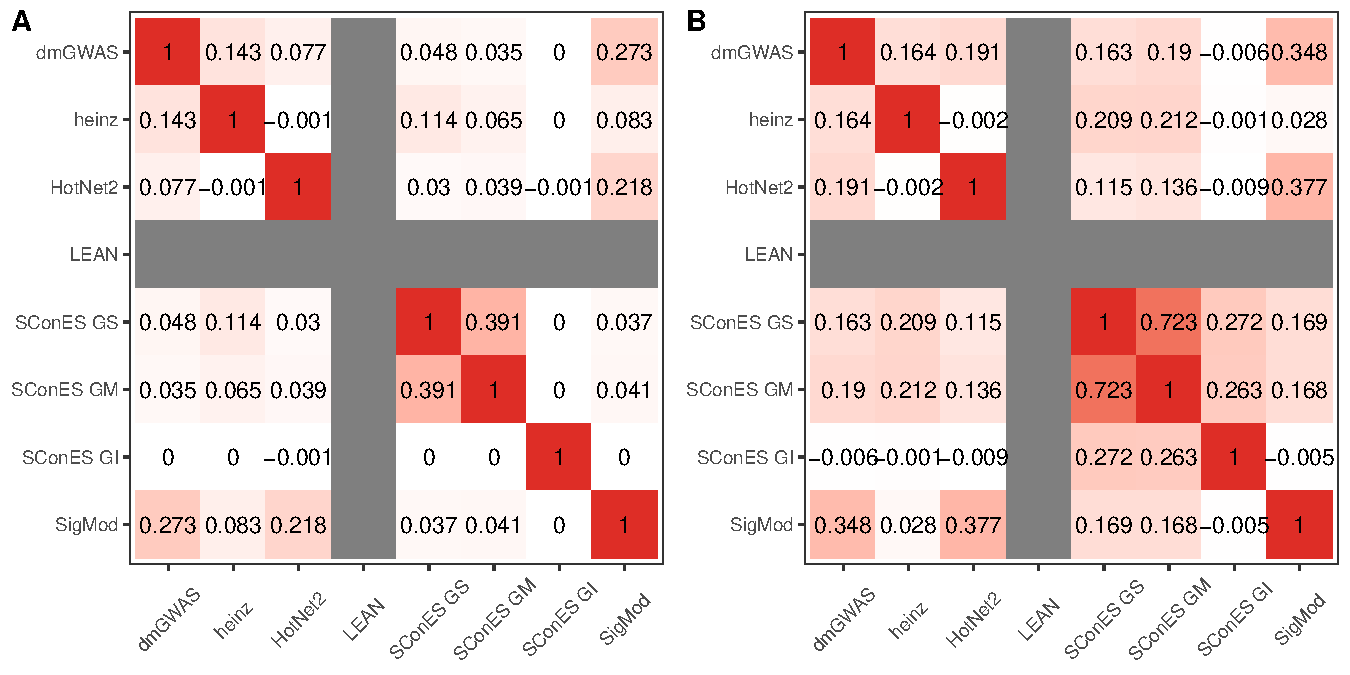
\includegraphics[width=.9\linewidth]{./figures/sfigure_6.pdf}
\caption{\label{sfig:biotypes_excluded}
Biotypes of genes from the annotation that are not present in the HINT protein-protein interaction network.}
\end{figure}

\begin{figure}[htbp]
\centering
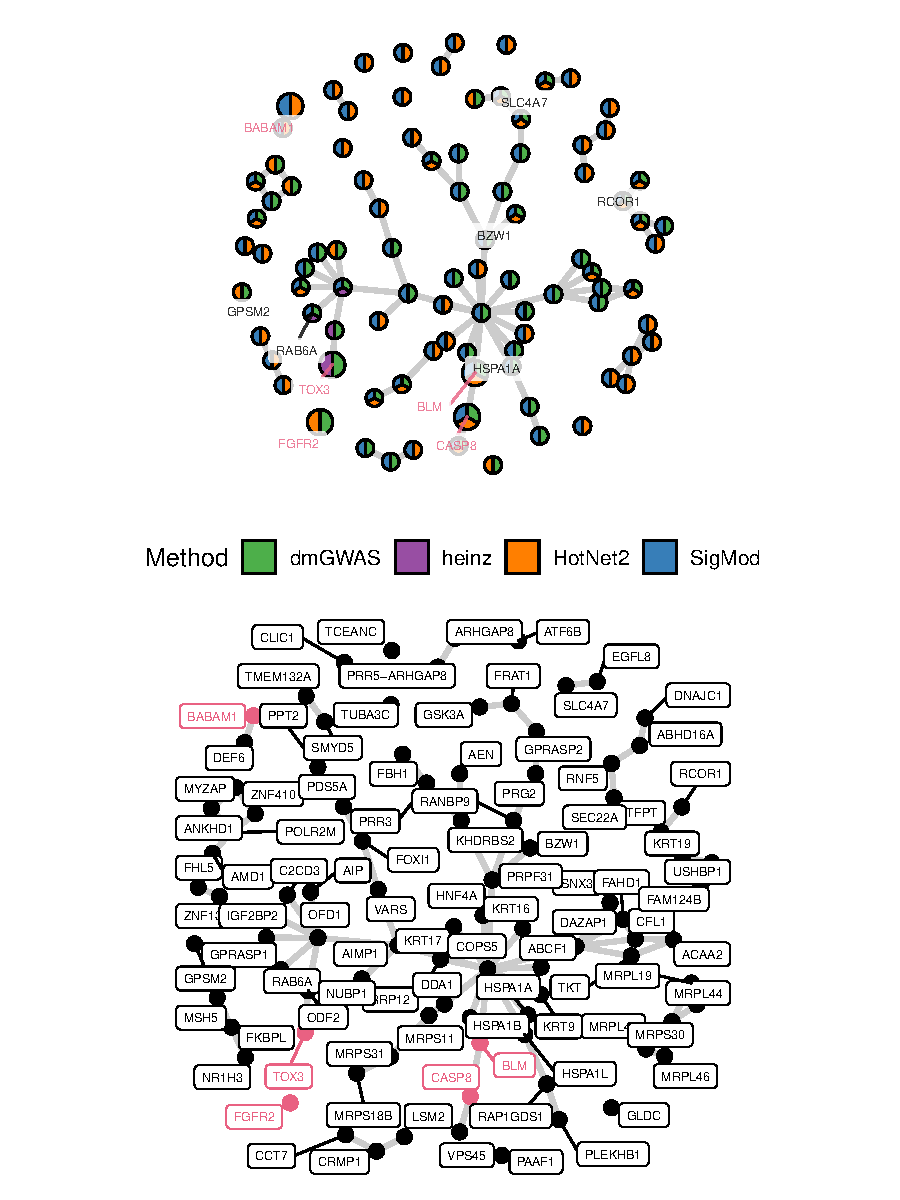
\includegraphics[width=.9\linewidth]{./figures/sfigure_7.pdf}
\caption{\label{sfig:lc_ht_comparison}
Comparison of benchmark on high-throughput interactions to benchmark on both high-throughput and literature curated interactions. Grey lines represent no change between the benchmarks (1 for ratios, 0 for differences). \textbf{(A)} Ratios of the selected features between both benchmarks and of the active set. \textbf{(B)} Shifts in sensitivity and specificity. \textbf{(C)} Shift in Pearson's correlation between benchmarks. \textbf{(D)} Ratio between the runtimes of the benchmarks. For gene network-based methods, inverted triangles represent the ratio of runtimes of the algorithms themselves, and circles the total time, which includes the algorithm themselves and the additional 119\,980 seconds (1 day and 9.33 hours) which took VEGAS2v2 on average to compute the gene scores from SNP summary statistics. In general, adding additional interactions slightly improves the stability of the solution, but increases the solution size, has mixed effects on the sensitivity and specificity, and impacts negatively the required runtime of the algorithms.}
\end{figure}

\begin{figure}[htbp]
  \centering
  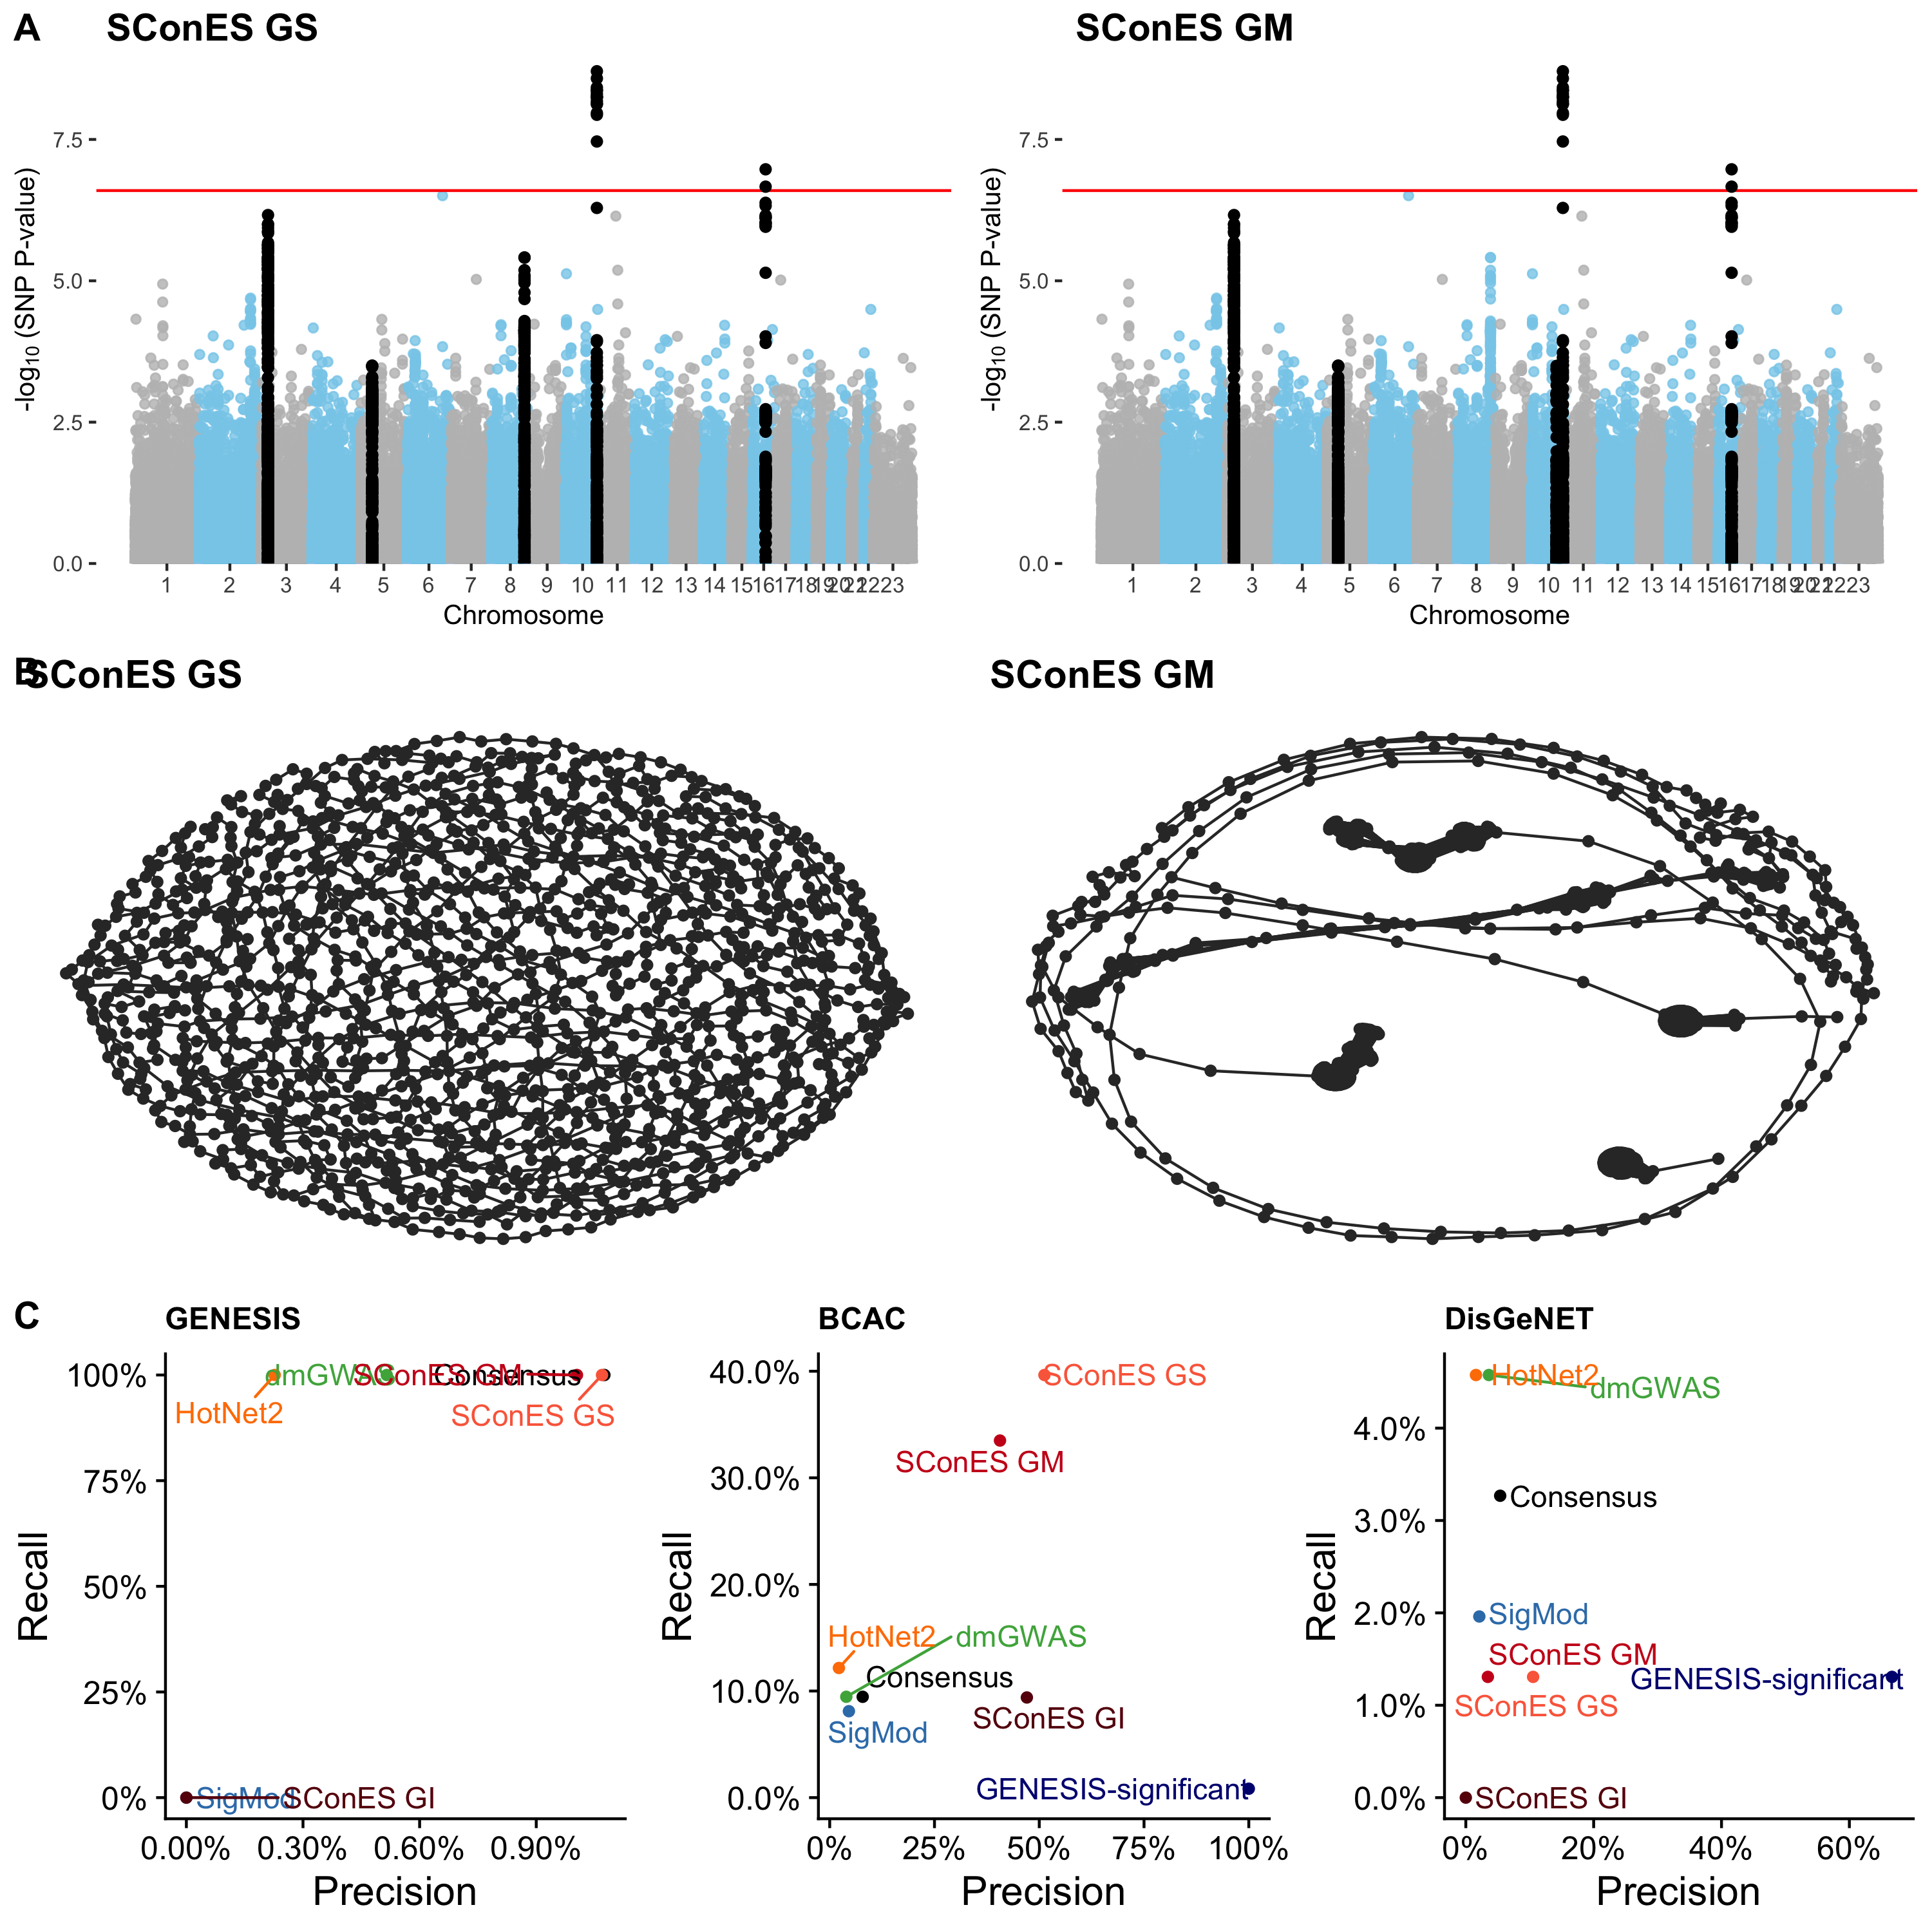
\includegraphics[width=.9\linewidth]{./figures/sfigure_8.png}
  \caption{\label{sfig:scones_gsm} TODO.}
\end{figure}

\end{document}
